% !TEX root=frame_thesis.tex
\chapter{Results and Discussion}\label{chapter:Results}
\FloatBarrier
\section{A Standard Run}
%\paragraph{Aggregate Dynamics of Trees and Population}
%\paragraph{Spatial Pattern at different time snapshots}
\paragraph{Overview of the Results.}
The standard run of the ABM presented in Section \ref{chapter:Methods} 
is set up with parameters as described in Table \ref{tab:sensitivity}.
%proofs the general functioning and consistency of the model with the generally expected behaviour of the socio-ecological system.
Snapshots of the spatial pattern of trees, farmed sites, and agents (with their tree preferences) at different times are shown for one simulation in Figure \ref{fig:STDrull}.
In the supplementary material, I provide a link to an animated Figure showing these spatial patterns of a single simulation over time.
Since multiple processes in the model are stochastic, each run with different seed is only a single realisation.
In order to obtain statistically valid aggregate results, I use an ensemble of $15$ runs for all experiments.
Adding more runs (e.g.\ 20 or 25) does not significantly change the coefficient of variation for the ensemble over time (see Figure \ref{fig:coeffofvariation}).
The mean and standard deviation of the aggregated variables of this ensemble and their change over time is shown in Figure \ref{fig:STDstats}.
The uncertainty in the ensemble runs results from slight differences in the timing of the dynamics due to different realisations of the discrete, stochastic population growth process (see also Figure \ref{fig:realisationsofpopgrowth}). 
Hence, the peaks of the population sizes of single runs are at a similar level but temporally shifted. 
The ensemble mean therefore slightly underestimates the peak population size.

\begin{figure}
	\centering
	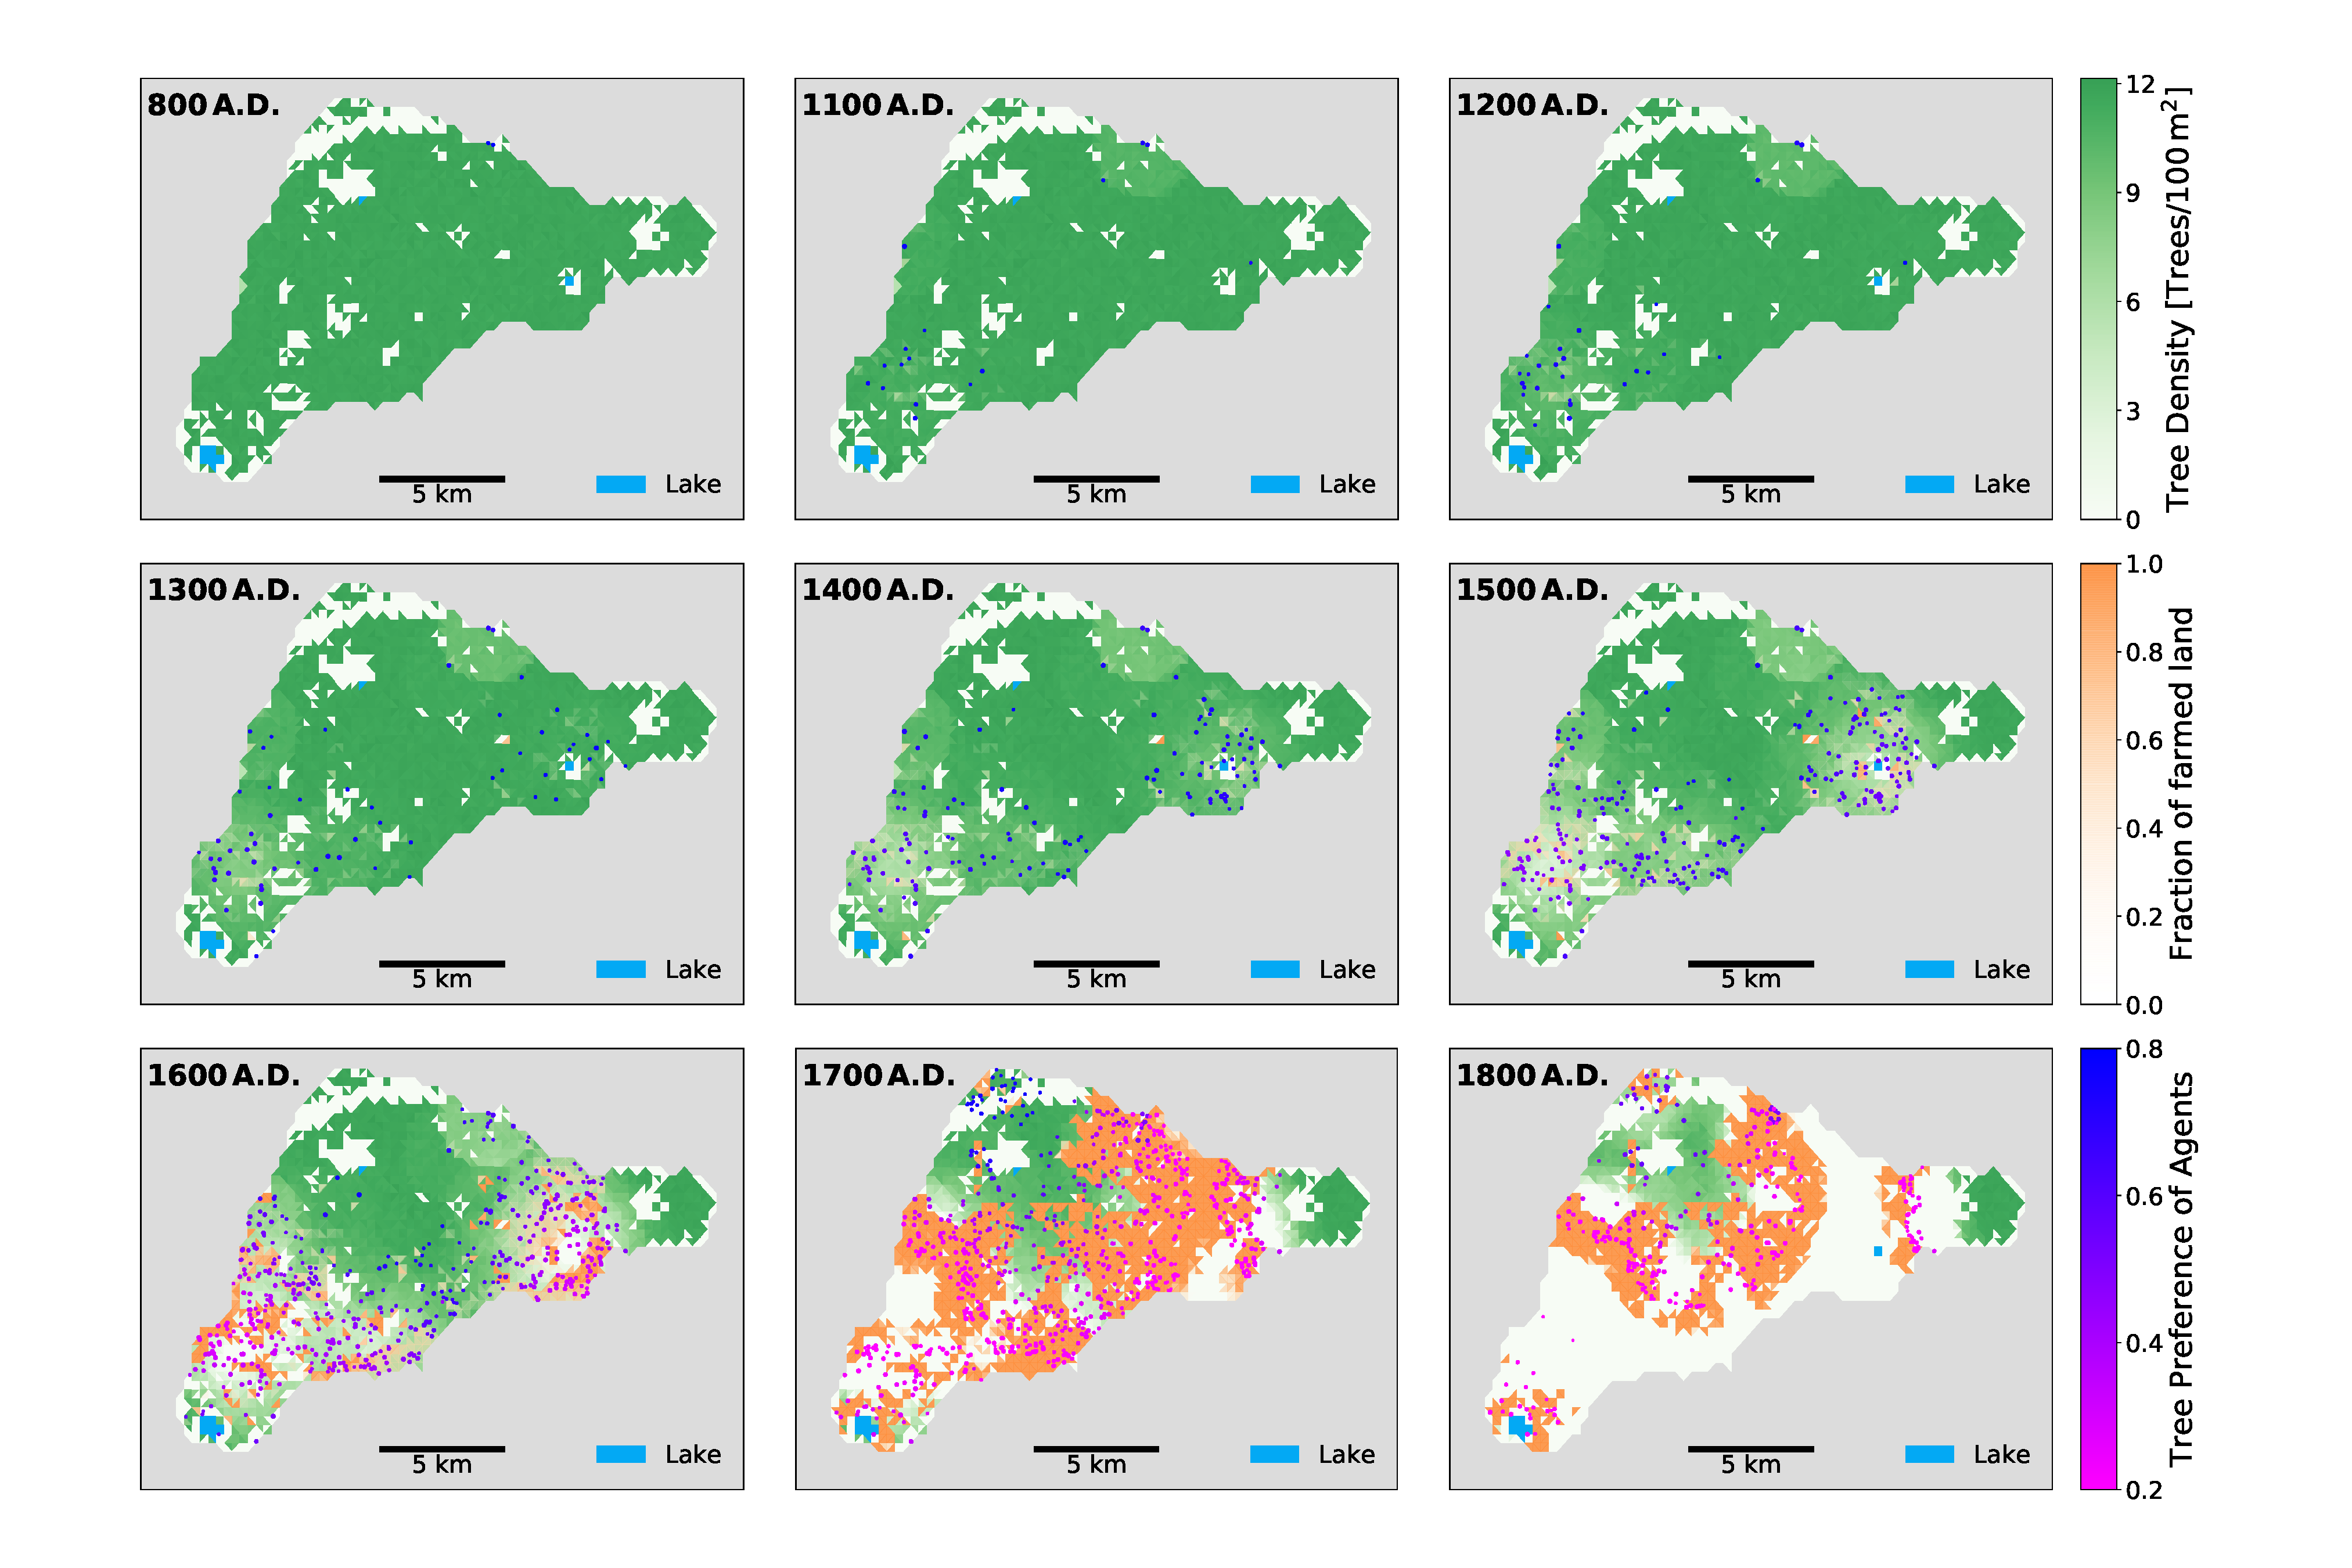
\includegraphics[width=1.3\textwidth, center]{images/Results/Standard/Rull2020_Comparison_seed3}
	\caption{The spatial patterns of Easter Island ABM for snapshots at nine different times (comparable to Figure 9 in \citen{Rull2020}). The map shows the tree density in green and the fraction of farmed land in orange. Agents settle on the island and interact with the environment by cutting trees and turning arable land into farmed sites. They are represented by dots with a colour corresponding to their tree preference and size corresponding to their population size.}
	\label{fig:STDrull}
\end{figure}


\begin{figure}
	\centering
	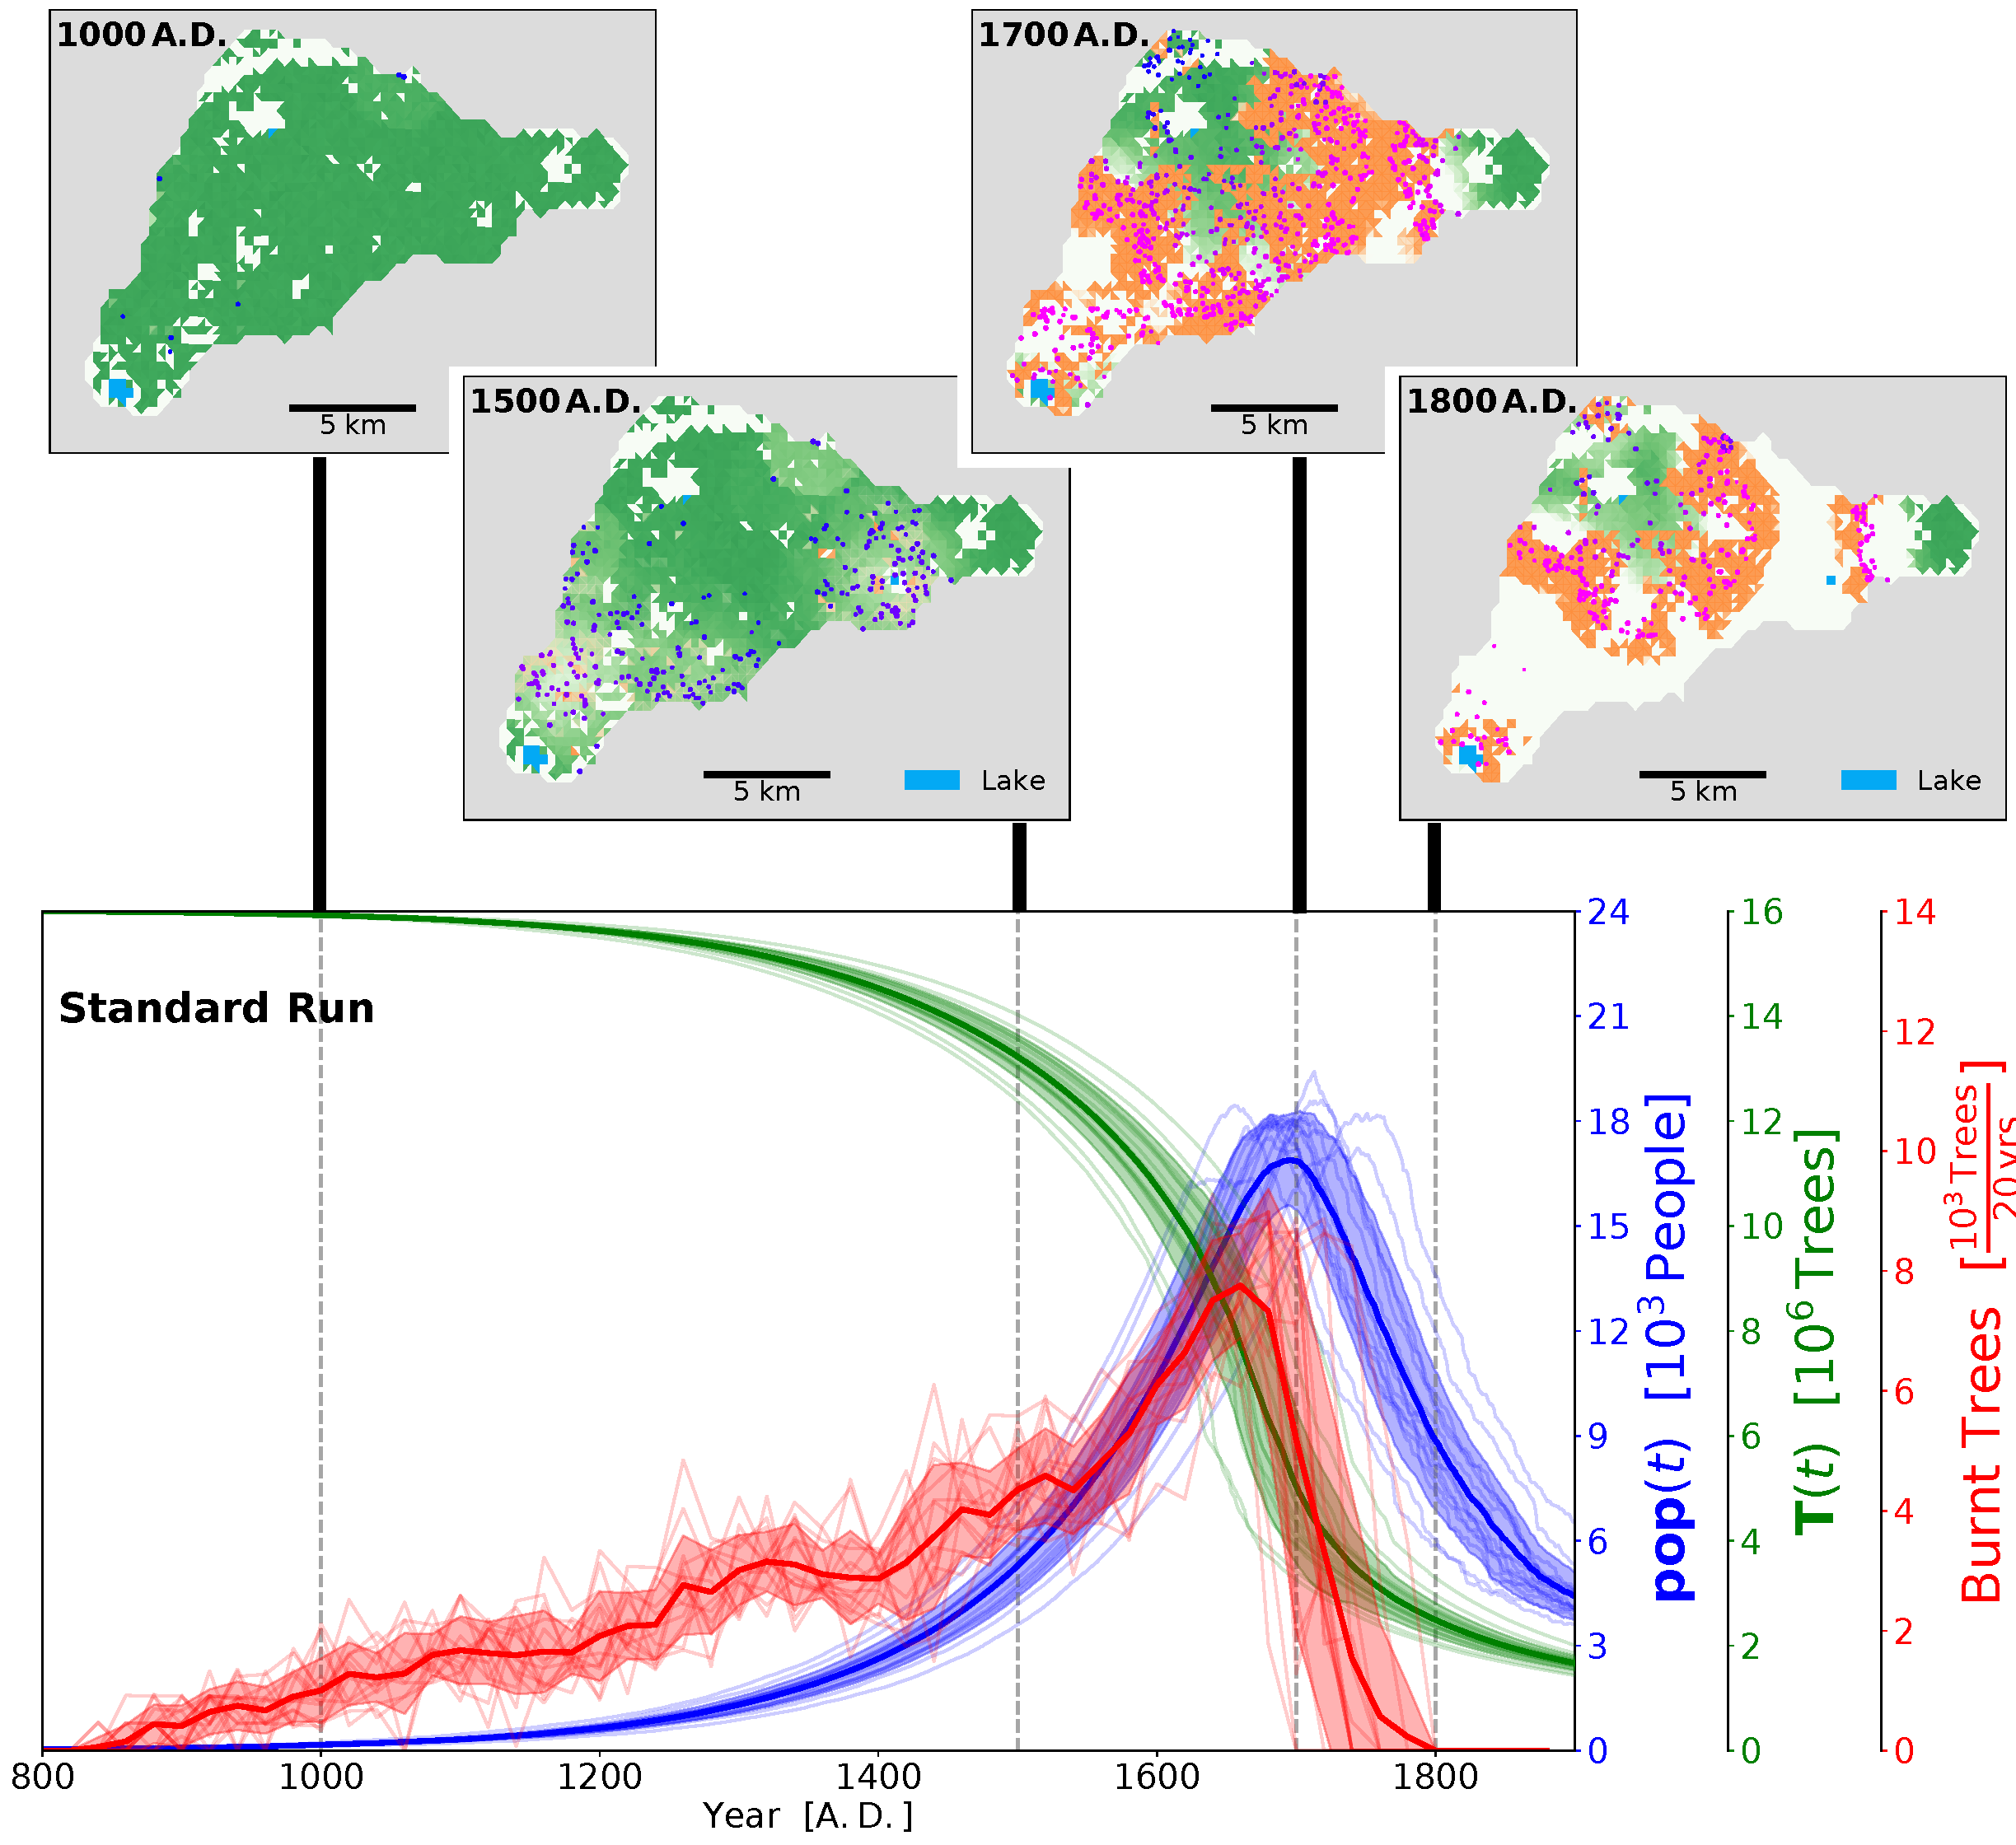
\includegraphics[width=1.\linewidth, center]{images/Results/Standard/EnsembleStatistics+Panels}
	\caption{Dynamics of aggregate population size, trees, and burnt trees with standard setting of parameters. 15 different realisations (thin lines) are used to obtain the ensemble mean and standard deviation (shaded area). The panels above show the spatial distribution of trees, farming and agent settlements with their tree preferences for one of these realisations (with the same colour coding as in Figure \ref{fig:STDrull}).}
	\label{fig:STDstats}
\end{figure}


\paragraph{The first phase: Initial Growth.}
In the beginning of the simulation agents settle at Anakena Beach (in the North). 
The local tree density is at the carrying capacity and thus the agents' tree preference is high (blue colour in Figure \ref{fig:STDrull}).
In the first phase of the simulated time period, the agents' population size grows at a constant maximum growth rate, because trees and arable land are both abundant. 
Consequently, groups of individuals split, form new agents and start to colonise the rest of the island. % according to the penalty evaluation scheme described in Section \ref{sec:Moving}.
Until the end of the first drought period in $1200\, {\rm A.D.}$, new agents tend to settle in the arable, coastal region South/South East of the island close to the major freshwater source Rano Kau. 
%With population density on the rise, deforestation and farming activity in this region intensify.
After $1200\, {\rm A.D.}$, also the region around Rano Raraku (in the West), now providing an alternative, low elevation freshwater source, is settled at rapid pace.
%At $1200\,{\rm A.D.}$, the drought period ends and Rano Raraku (in the West) provides another freshwater source, causing many new agents to move to the South West and North West coast.
%With ever increasing population density, especially in these centres, 
Agents linearly adapt their tree preference to the slow environmental change and, thus, intensify farming activity.
As Figure \ref{fig:STDstats} shows, the amount of burnt trees to clear land for agriculture in a $20$ year time window also increases linearly in this phase.
%, followed by a sharp increase around 1650.
%At peak, roughly $10\cdot 10^3$ trees are cleared in a 20 year period in order to fill the agents' farming requirement.

\begin{figure}
	\centering
	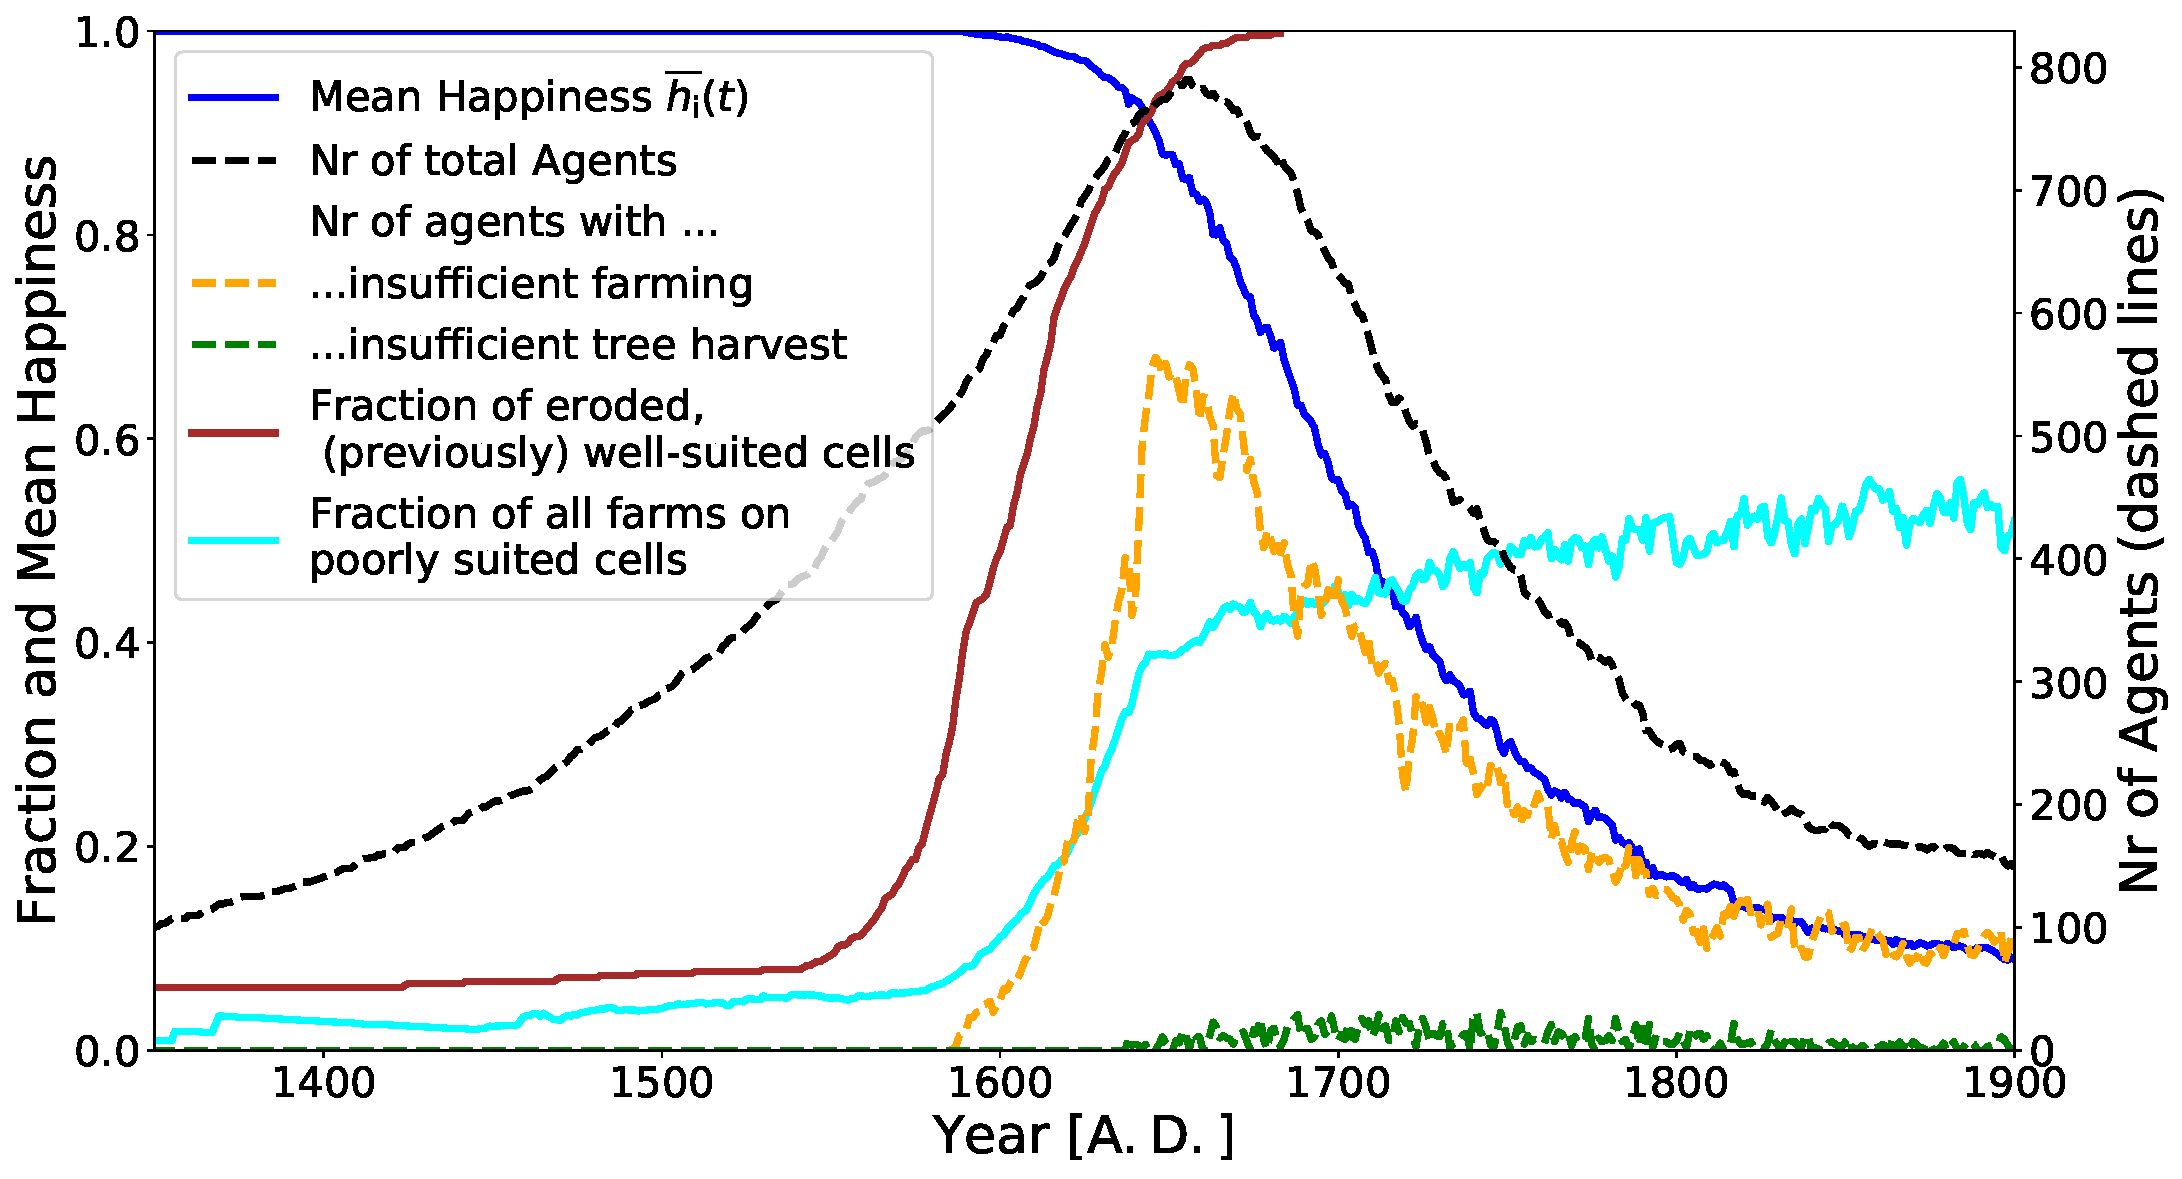
\includegraphics[width=\textwidth]{images/Results/Standard/StandardsecondaryStats}
	\caption{The plot shows the development and causes of the change from net growth to net decline in Easter Island population dynamics for one single realisation in the Standard setting.
	Dashed lines correspond to the axis on the right giving absolute number of agents.
	The blue line shows the mean happiness index of all living agents. The black, dashed line shows the total number of agents. The number of agents that lack either sufficient available land for farming or trees are shown in yellow and green, respectively. The brown line shows the fraction of cells that previously classified as well-suited for farming but has eroded due to complete deforestation. The cyan line shows the fraction of farming sites (of all agents) on poorly suited sites.
	The development is described in detail in the main text.}
	\label{fig:STDsecondayrstats}
\end{figure}

%Thereby, agents accelerate the depletion of the non-renewable resource, trees and, thus, in a self-enhancing loop, acquire more farming land.

%Further, this large-scale deforestation leads to a sharp increase of erosion of well-suited sites around $1650\, {\rm A.D.}$ and, hence, agents can not fill their farming requirements.

% with the first agents not meeting their resource requirements.
%However, since both neither further arable sites are available in the densely populated coastal regions and trees are deforested entirely by the remaining agents, these previously well-suited settlement locations are abandoned and the agents turn to the mostly poorly suited upland areas causing a shift towards the interior of the island.
%With the first agents not meeting their farming requirements around 1650, occupation of upland poorly suited farming sites jumps from a negligible fraction in $1650$ to $40-59\%$ in 1700.
%Consequently, the amount of burned trees rises quickly and comes to a abrupt halt between 1700 and 1800.
%Due to the low productivity indices of these sites, the use of burning trees to clear more space rises sharply in this period.

\paragraph{The second phase: Acceleration.}
The second phase of the dynamics is characterised by accelerating, non-linear feedbacks in several indicators shown in Figure \ref{fig:STDsecondayrstats}.
In a self-enhancing loop, population growth in the settlement centres leads to an intensification of deforestation, a consequent decrease of the agents' tree preferences, increase of farming requirements, more acquisition of farming sites (therefore, more burnt trees) and, ultimately, again more intense deforestation.
Simultaneously, erosion accelerates the deforestation as the farming productivity of occupied land decreases and  more needs to be acquired.
%of arable farming land increases, leading to declined farming efficiency and, thus, more farming sites required per agent.
The number of eroded, (previously) well-suited cells jumps from less than $10\%$ of all well-suited sites in $1600\,{\rm A.D.}$ to $100\%$ by $1700\, {\rm A.D.}$ (brown curve in Figure \ref{fig:STDsecondayrstats}).
Consequently, in this period the amount of trees burnt for clearing new land rises sharply. %to roughly $8\cdot 10^3$ trees per $20 \, {\rm yrs}$.
In total, this acceleration of the local resource scarcity, leads to an abandonment of the previously used well-suited settlement locations (nearly $100\%$ of all farming activity in $1650\,{\rm A.D.}$) and the agents turn to the mostly poorly suited, interior, upland areas (accounting for $40\%$ in $1700\,{\rm A.D.}$, cyan line).
%The share of farming activity on those poorly suited cells rises from a negligible fraction in $1650\, {\rm A.D.}$ to $40\%$ of all farming activity in $1700\,{\rm A.D.}$ (cyan line in Figure \ref{fig:STDsecondayrstats}).
%However, there is no year in which all available farming sites are occupied simultaneously.
%However, the lower productivity indices in the poorly suited sites, leads to a further increase in land acquisition and, thus, deforestation. 

\paragraph{The third phase: Population Decrease.}
The third phase is characterised by a population decline and substantial shift in the settlement patterns.
While in $1700\,{\rm A.D.}$ more than half of the agents experience some minor shortage in farming produce (yellow curve in Figure \ref{fig:STDsecondayrstats}), 
%there is no time when all arable spaces are farmed simultaneously.
the loss of the non-renewable resource, trees, experienced by only a few agents each year (green line in Figure \ref{fig:STDsecondayrstats}) triggers an exponential decline of the averaged happiness, $\overline{h_{\rm i}(t)}$, just after $1700\, {\rm A.D.}$ (blue line in Figure \ref{fig:STDsecondayrstats}).
This sets on a period of excessive moving.
Figure \ref{fig:penaltiesag500t1603} shows an example of an agent's penalty evaluation while searching for a new settlement location.
\begin{figure}
	\centering
	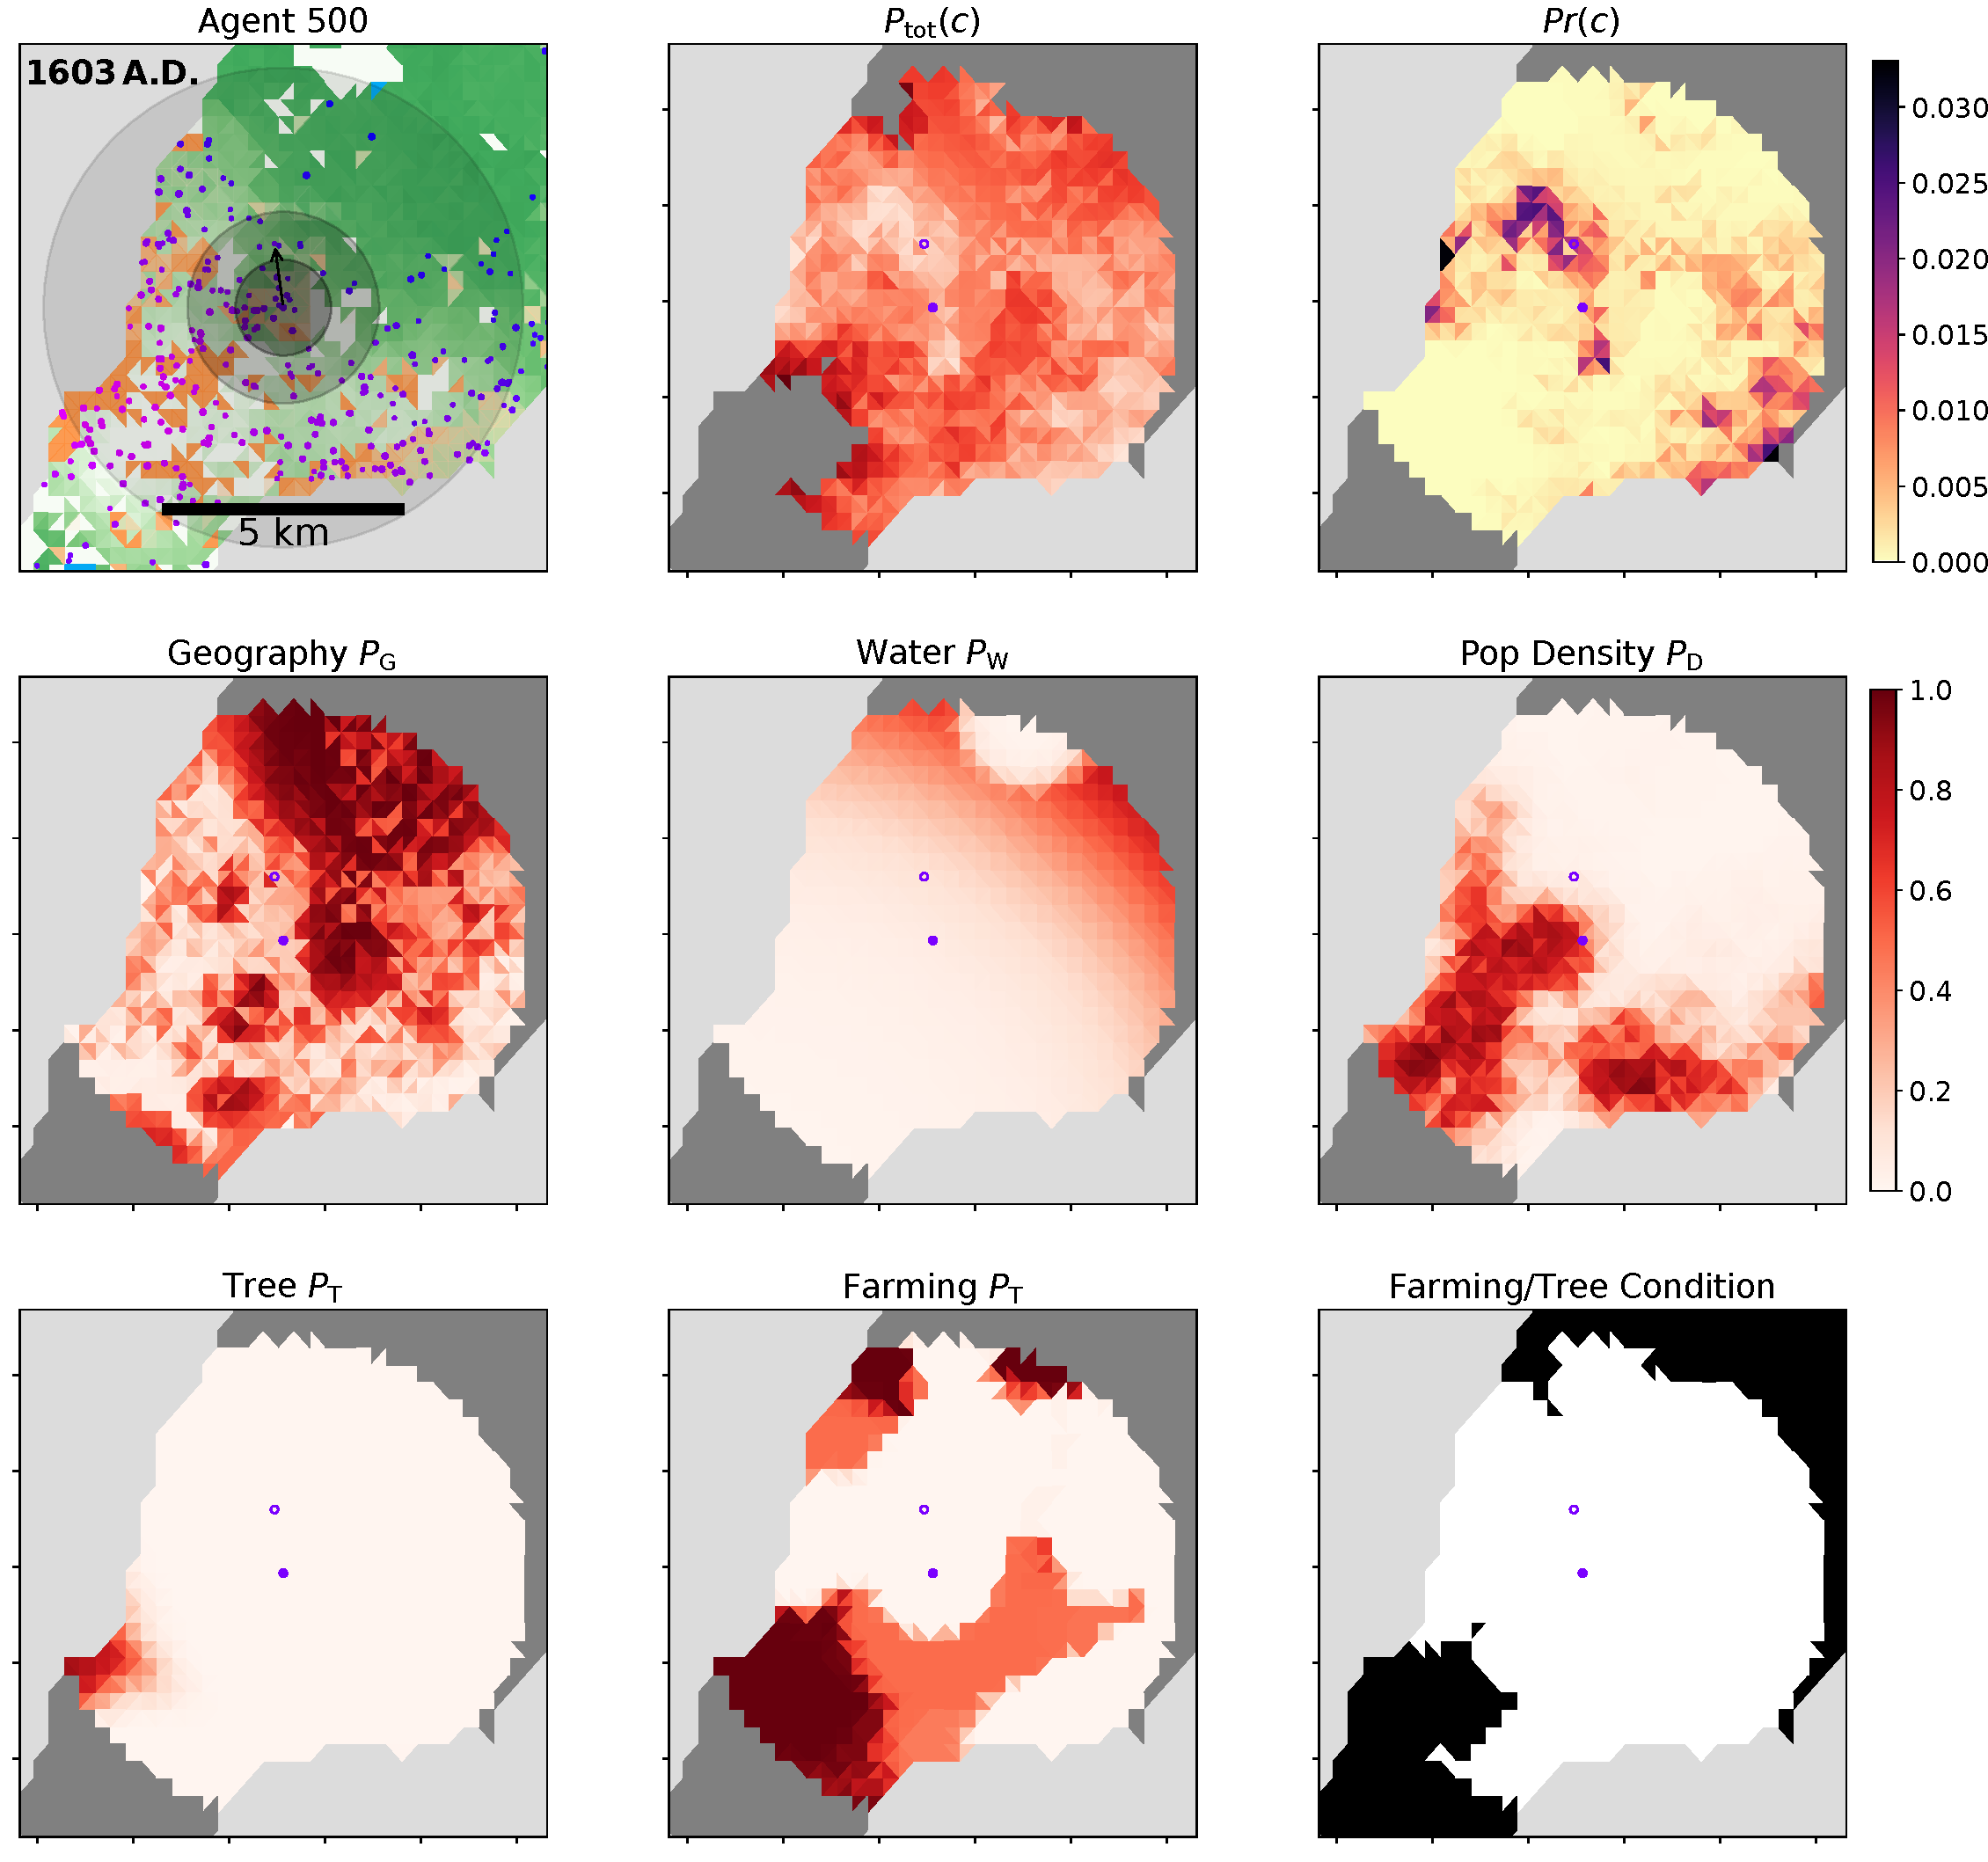
\includegraphics[width=1.3\linewidth, center]{images/Results/Standard/Penalties_AG500_t=1603}
	\caption{Decision making in the moving module of an agent at time $1603\, {\rm A.D.}$ located in the South East. 
		Each panel shows the same region of interest with the old location of the agent in the centre (filled dot) and the new location after the decision making (unfilled dot).
		The upper left panel shows the agent in its current local environment, indicated by circles with the radii $r_{\rm F}$, $r_{\rm T}$, and $r_{\rm M}$ (after the moving restriction). The upper middle panel shows the total penalty ($\in [0,1]\cup \infty$), and upper right the corresponding probability for the agent to move to each allowed cell. The remaining panels show the penalties in all categories ranging from $0$ to $1$.
		The lower right panel also shows, which cells are excluded because the do not fulfil the necessary condition for tree and farming availability (black cells inside the $r_{\rm M}$ circle).}
	\label{fig:penaltiesag500t1603}
\end{figure}
The development in this phase also marks the end of the net exponential growth of the population size, which peaks at around $18\cdot 10^3$ people.
Within a relative short time period of less than $50$ years, the population starts to decrease exponentially with a growth rate of $-0.5$ to $-1\%$ (see Figure \ref{fig:app:STDnetgrowthrate} in the Appendix).
There is neither insufficient total area of farming land (there is no year in which all arable sites are farmed simultaneously), nor insufficient total number of trees on the island.
However, since the harvest is confined to the local surrounding, agents in a specific location lack one or the other resource and at some point there are no valid locations left that fulfil both resource requirements.
Consequently, an agent's eoffective happiness, $H_{\rm i}(t)$ quickly drops to $0$ and the overall population size decreases.
As a result of the decreasing population size, the deforestation level slows down around $1750\, {\rm A.D.}$ at slightly less than $25\%$ of the initial total number of trees. 
%have not enough farming sites with a happiness $H_{\rm i}(t)>H_{\rm equ}$ and therefore positive net growth. 
%The agents unable to find enough trees to cut, however, at this point of time quickly vanish as there are no valid locations to settle anymore and no replacement leading to a memory happiness of $H_{\rm i}(t) = 0$ very quickly.
%Finally, by $1800\,{\rm A.D.}$, the population decrease slows down. 
%The net population growth is shown in Figure \ref{fig:app:STDnetgrowthrate}. 
However, there is no stable coexistence of population and trees in this scenario setting as tree regeneration is disabled and, hence, the agents rely on an entirely non-renewable resource and vanish completely as it becomes exhausted.


\paragraph{Outcomes Consistent with Ecocidal View.}
The succession of events in the standard run presented here follows a boom and bust scenario consistent with the classical narrative of Easter Island history of a Malthusian catastrophe initiated by overexploitation supported by \citet{Brander1998}, \citet{Diamond2011} or \citet{Bahn2017}.
This is not surprising as the agents are designed to maximise their personal population growth every year but eventually rely on a non-renewable resource and a limited, renewable resource.
Furthermore, the arrival date and initial population growth are taken from the ecocidal narrative.


\paragraph{Caveat: Population Size is Maximised Myopically per Definition.}
In general, the population size in this model is at the upper range of most estimates stated in the literature \citep{Bahn2017}.
This is partly due to the fact, that there is no restriction on the amount of labour that agents can put into the resource acquisition. 
Also, the model does not include any social development or political institution e.g.\ to stabilise the population growth or harvest of natural resources via taboos.
Further, I assume that except for the eventual erosion of all well-suited cells, arable land has a constant, entirely predictable crop output (in particular even constant during the drought periods). 
Land availability is, thus, the only constraint for agricultural production. 
%\todo{A certain stochastic variation due to different climatic conditions each year could be implemented into the model.}
Sustainability criteria concerning the resource availability (locally and island-wide) do not play a role in the agents' myopic, unabated population expansion as long as the resource situation allows it.
Agents here also do not plan ahead while harvesting e.g.\ trees could be cut first (e.g.\ for extracting the sugary sap) and then burned to clear the land for farming next year as indicated by \citet{Mieth2015}.
Only when resources become scarce, the population growth declines and turns negative.
Hence, the peak size is maximised and a (strong) consequent decrease inevitable as agents are determined to overexploit.


\paragraph{The Spatial Component.}
As a first mathematical modelling approach, this model quantitatively investigates the spatial component of the Easter Island settlement history emerging from the local harvest behaviour and moving decisions by the agents.
The results show strong agreement of the obtained tree densities (Figure \ref{fig:STDrull}) from this model in the comparison with a qualitative sketch of tree density obtained from charcoal and pollen data of the three crater lakes in \citet{Rull2020} (Figure 7 and 9) including anthropogenic and natural drivers (which are not considered here).
Additionally, throughout the entire book, \citet{Bahn2017} describes a qualitative phase sequence of the spatial Easter Island settlement history which also fits well to the obtained emergent patterns in this study:
Settlement of some coastal regions (especially South East Coast near Rano Kau and Anakena Beach) ($800$ to $1100\, {\rm A.D.}$), settlement of the whole coast ($1100-1425\,{\rm A.D.}$, with South Coast rising rapidly around $1300\, {\rm A.D.}$), population and farming peak ($1425-1680\, {\rm A.D.}$), and, finally, population reduction and remote fields abandoned ($1680\,{\rm A.D.}-$ European contact).
%In an early phase ($800$ to $1100\, {\rm A.D.}$) the settlers centred near the coastal area, especially in the South West near Rano Kau. Anakena Beach was settled some time before $1000\, {\rm A.D.}$. 
%Between $1100-1425\,{\rm A.D.}$ the whole coast was occupied with the South Coast experiencing a rapid build up around $1300\, {\rm A.D.}$. First inland field systems are established and the megalithic cult of building the Moai starts.
%The population and farming peaks in $1425-1680\, {\rm A.D.}$. Followed by a last phase, in which population reduces and remote field systems are abandoned.
While this spatial timeline is only consistent with the ecocidal narrative and should be treated with care, the standard run in this ABM presented here captures most of these qualitative statements\footnote{except for the abandonment of the remote fields during the population decrease}.



%Next to the aggregate dynamics, the model also mostly replicates the qualitative, spatial history given by \citet{Bahn2017}.
%According to this, in the initial phase the population centered around the Hanga Roa area near Rano Kau, \TODO!

%Furthermore, the model produces spatio-temporal data of deforestation level, which can be compared to actual data.
%By analysing pollen and charcoal records in the three crater lakes, \citet{Rull2020} provides a temporal history of the tree densities in the near surrounding of the three lakes over time. 
%With this model I can simualte the island-wide tree density emerging from the population size dynamics and complex agent harvest and moving behaviour.
%The result is  Figure \ref{fig:STDrull} in this thesis in comparison with Figure 9 in \cite{Rull2020}.
%In general, the dynamics of the model (despite no natural variability) is well replicated.
 
%especially cultivation of poorly suited sites, which in turn increases the fires and amplifying the development.
%In turn, sharp increase of fires around $1600\, {\rm A.D.}$. 
%Around $1650\, {\rm A.D.}$, constant exponential growth stops, population size remains constant for a short period and, finally, decays exponentially.
%This coincides with a steep increase of agents with not enough available farming productivity causing the mean happiness to decline. 
%As shown in Figure \ref{fig:happyStd}
%However, only when trees become scarce in the region



% \begin{itemize}
% 	\item Fig 2: Aggregate Dynamics (population, trees, mean penalties and happiness, fires, excess mortality/fertility). The plot that Esteban sketched during last Zoom Meeting [called statistics plot from now on]. All statistics plots are mean ensemble runs of 5 different seeds.
% 	\item Fig 1: Comparison of the spatial deforestation pattern with \citet{Rull2020}'s Figure, which we sent to Valenti.
% \end{itemize}


%The dynamics of population size $\mathbf{pop}(t)$, total number of trees $\mathbf{T}(t)$ and amount of burnt trees in a 20 year time period) are shown in Figure \ref{fig:STDstats}. 
%For the first $850\, {\rm yrs}$ after arrival, the population grows exponentially.
%Then, around $1650\, {\rm A.D.}$ the dynamics change significantly, leading to a significant population size reduction after $1750\, {\rm A.D.}$.
%The rate of population size decrease is ....\TODO (i.e.\ the number of $g(H_{\rm i}(t))$ for agents $i$ and $t>1750\, {\rm A.D.}$ is on average ... \TODO.).vanish


%
%We can look 
%Figure \ref{fig:app:treefillfarmfillmoves} 



%\section{Dynamics in Separate Regions in the Standard Run}
%\paragraph{Quantitative Analysis Approach}
\paragraph{Temporal Dynamics in Separate Regions.}
There is strong regional variation in the dynamics of the population as well as the deforestation as qualitatively shown in Figure \ref{fig:STDrull}. 
To quantitatively analyse these different developments, I divide the island into seven different regions with common geographical features (Figure \ref{fig:mapregionscoarse}): The area around the crater lake Rano Kau, the South Coast, Rano Raraku, Anakena Beach, the steep North West Coast, the fertile area covering today's main town, Hanga Roa, and the upland area including Poike Peninsula. 
By choosing centre points of each region or several sub-regions on the map by hand, a region is defined by the cells allocated to the corresponding Voroni Diagram.

\begin{figure}
	\centering
	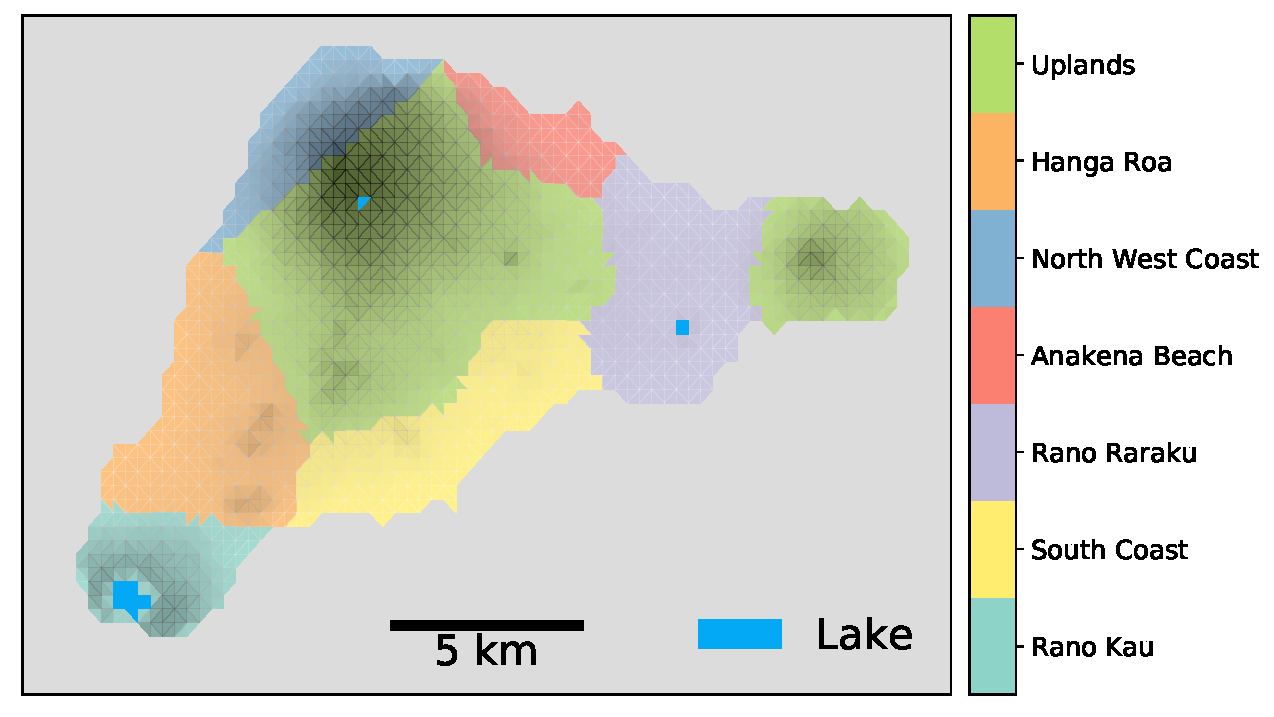
\includegraphics[width=1.0\linewidth]{images/Results/Standard/MapRegionsCoarse}
	\caption{Division of the map into seven separate regions. The black shadow represents elevation.}
	\label{fig:mapregionscoarse}
\end{figure}
Figure \ref{fig:regionalstats} shows the results of the population in each region over time in the ensemble of 15 runs.
Overall, the island shows diverse and heterogeneous population dynamics. 
Some regions, like Hanga Roa and the South Coast (with a little delay), show early extensive growth followed by a steep decline of the population size.
The population around Rano Raraku grows nearly linearly and then, as in the Uplands, declines less strong after reaching the peak.
In some single realisations, this effect is more pronounced than in the ensemble mean.
The small, less arable regions at Rano Kau, the North West Coast, or Anakena Beach, show some population growth following the abandonment of other, more favourable regions.
The population size in these regions then either declines close to linearly or even remains at the same level for nearly $200$ years.
\begin{figure}
	\centering
	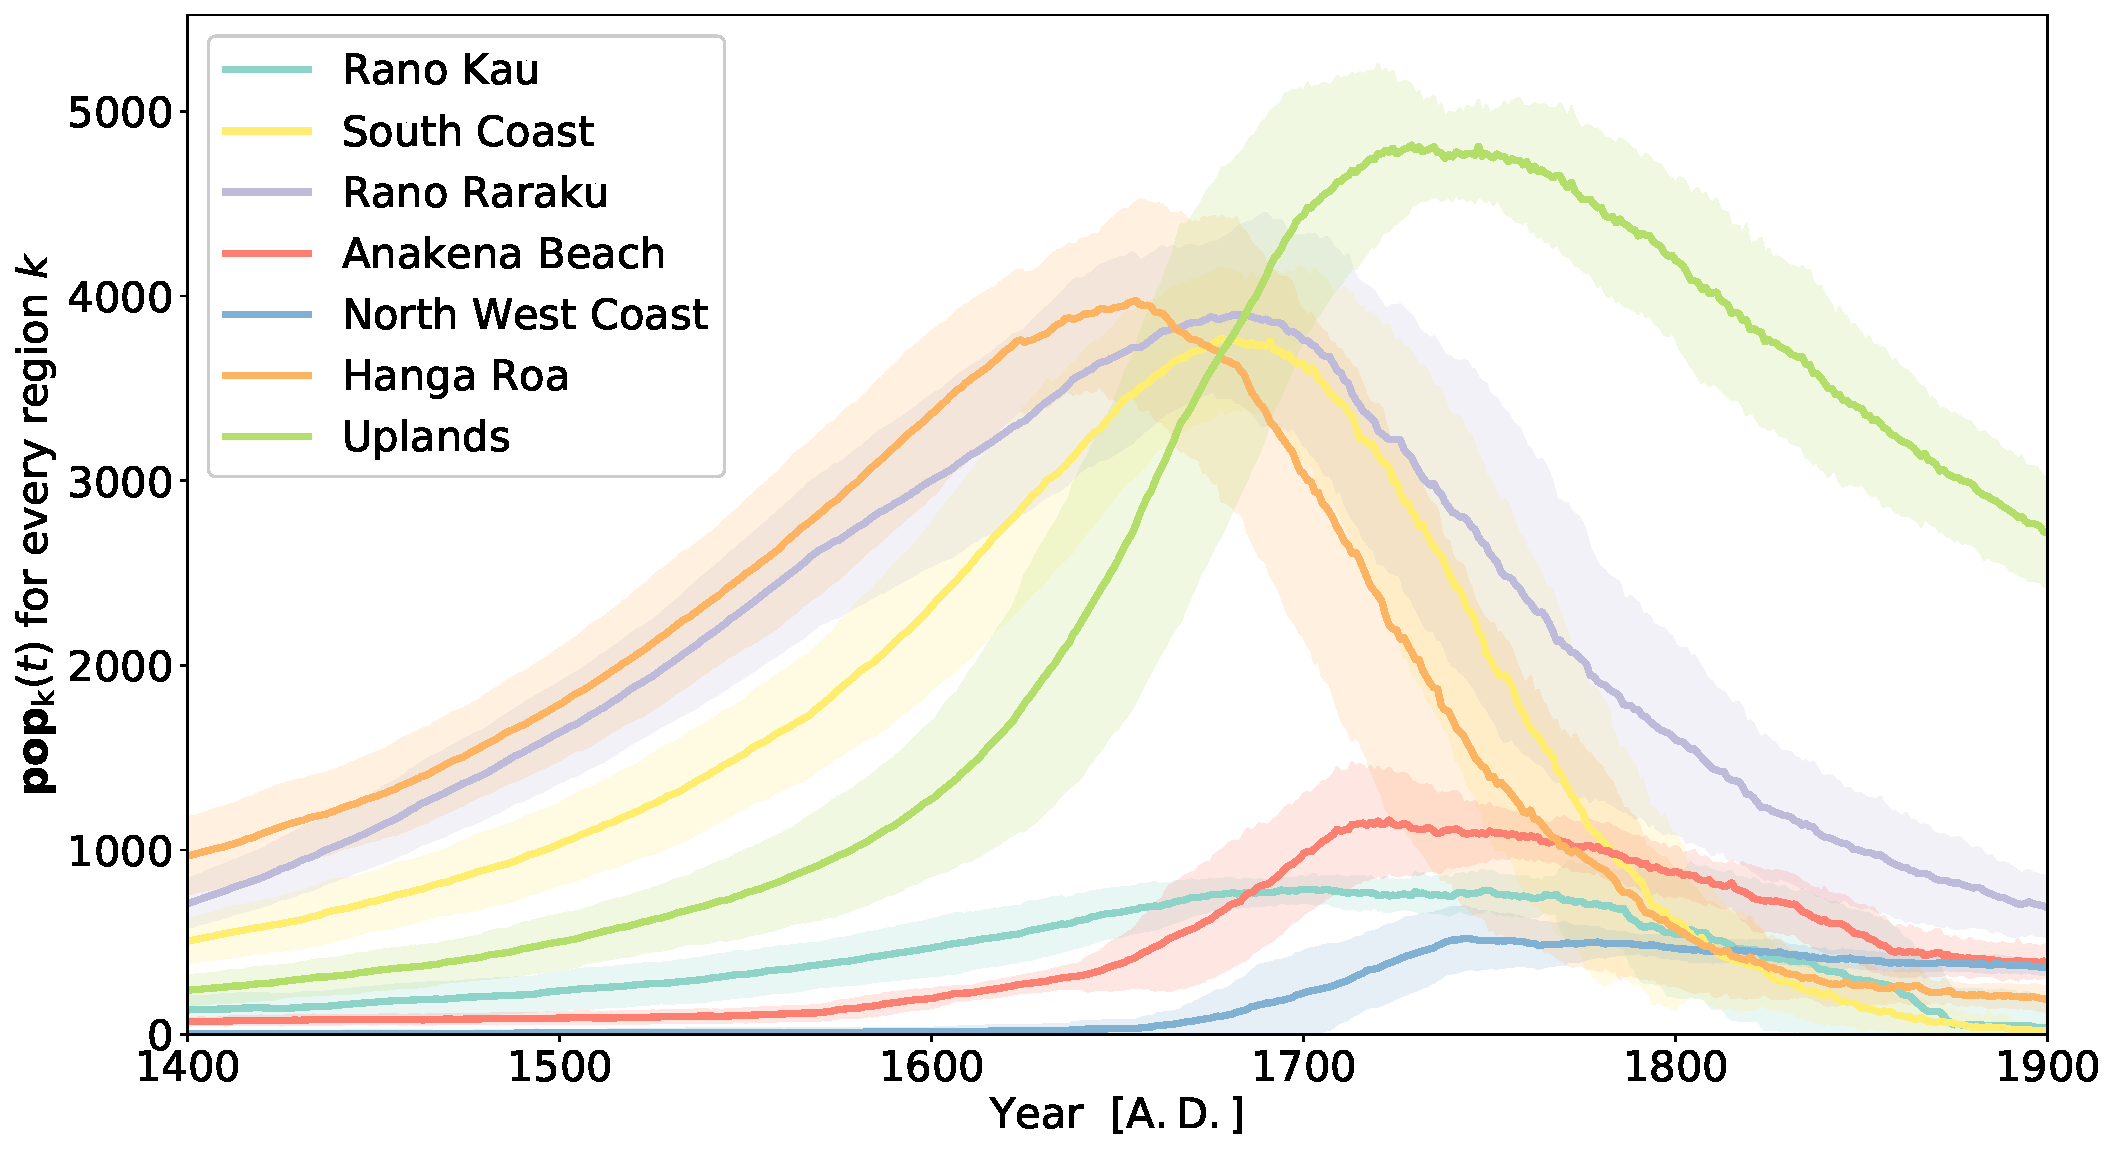
\includegraphics[width=1.0\linewidth]{images/Results/Standard/RegionalStatsEnsembleOnly}
	\caption{The population dynamics of each separate region defined in Figure \ref{fig:mapregionscoarse} as an ensemble of 15 single realisations.}
	\label{fig:regionalstats}
\end{figure}
Given this strong variation of the dynamics between different regions, this model makes a point in being careful about extrapolating data or conclusions about population dynamics based on information in single locations.
This ABM, though, could provide an indication of what such data could imply for the whole island.

\FloatBarrier
\section{Experiments and Sensitivity Analysis}

\subsection{Variation of Parameters Connected to the Abundance of and Requirements for Resources}
%\paragraph{Aggregate Dynamics for different choices of parameters mainly influencing the Total Population Dynamics --> Different theories of total population dynamics replicated}
%Statistics Plots for a
%\begin{itemize}
%	\item Run with low N fixation (instead of high)
%	\item Run with tree regeneration and high N fixation
%	\item Run with tree regeneration and low N fixation
%\end{itemize}
%In the making


\paragraph{Outcomes Consistent with Different Narratives.}
The standard parameter setting used for this model reproduces a boom and bust dynamics, with a population decline at a rate in the order of the initial growth rate following a short peak period.
However, the parameters in this setting are debatable and this uncertainty lies at the heart of the contrasting views of Easter Island's historical development.
In particular, the (spatially varying) farming yields on Easter Island soils (here expressed via $F_{\rm Req, \ pP}$ and, correspondingly, $F{\rm PI}(c)$) are uncertain.
Also, $T_\text{Req, pP}$ is speculative and in fact probably highly heterogeneous between agents.
These constant parameters, $F_{\rm Req, \ pP}$ and $T_{\rm Req\ pP}$, determine the amount of tree harvesting and farmland occupation and, thus, are crucial for the temporal development of the island's environment and the peak population size. 
In a series of experiments I change these constants, $F_{\rm Req, \ pP}$ and $T_{\rm Req\ pP}$, and/or additionally allow tree regeneration.
Figure \ref{fig:ensemblestatisticsalltheories} shows four different scenarios with strongly varying results:
\begin{itemize}
	\item The upper left panel is again the standard run (using the high Nitrogen fixation scenario in \citet{Puleston2017} for $F_\text{Req, pP}$ and disabled tree regeneration) shown in Figure \ref{fig:STDstats} for comparison.
	\item In the upper right panel, I choose the scenario with low Nitrogen fixation by \citet{Puleston2017}, i.e.\ agents have a higher requirement of farmed land per person.
	Population size (blue) peaks earlier and at a smaller number (ca. $6000$ people) and the consequent decrease is slower with a rate close to $-0.2\%/yr$.
	The amount of burnt trees (red) especially in the first phase with constant population growth rate is higher in this scenario, because more arable land needs to be occupied by the agents.
	\item In the corresponding bottom panels, tree regeneration is enabled with parameters set as in Table \ref{tab:sensitivity}. 
	For both cases with tree regrowth (lower panels), a heterogeneous pattern of agents with different tree preferences emerges with some areas dominated by agents at maximum, some at minimum tree preference (not shown here).
	\begin{itemize}
		\item In the lower left panel, with high Nitrogen fixation, a population of nearly $24\cdot10^3$ individuals is reached at a later time than in the standard setting. After that peak, the population size then declines slowly until an equilibrium between tree renewal and tree cutting is reached with all arable sites being occupied after $1700\, {\rm A.D.}$.
		There are two temporarily separated peaks in the amount of burnt trees around $1300\, {\rm A.D.}$ and $1650\, {\rm A.D.}$.
		\item In the lower right panel, with low Nitrogen fixation, population peaks at a similar level and time compared to the case without tree regrowth.
		Here, however, the population size remains constant roughly at this peak level with all arable sites being occupied before $1600\, {\rm A.D.}$.
	\end{itemize}
	%However, the peak population size occurs later and at respectively higher levels if the resource trees replenishes and the resource 
	%After reaching the peak, the population size decreases slowly and levels off at an equilibrium value for both scenarios, in which the renewal of trees matches the requirement of the population and the amount of farming land required remains constant.
	%In both cases with tree regrowth, all available arable sites are farmed in $1600\, {\rm A.D.}$ and $1700\, {\rm A.D.}$ (and mostly remain occupied throughout the rest of the simulation).	

\end{itemize}
A further experiment (not shown) with increased tree requirement per person $T_\text{Req, pP}(t)=10\,{\rm \frac{Trees}{yr\cdot person}}$ yields a similar boom and bust as in the standard setting but the population size peaks earlier and, thus, at a lower peak level ($\sim 13000$), and in general deforestation is intensified in this scenario.
 %(since trees do not regrow on cells with farms in the model or not regrow at all). 
 
The results of these different scenarios obtained by varying only two or three parameters resemble to some degree to the strongly contradictory storylines of prehistoric population dynamics.
The low Nitrogen fixation scenario\footnote{consistent with \citet{Hunt2007}'s assumption of low quality soil} resulting in constant or only slowly decreasing population size decline corresponds more to the genocidal \citep{Hunt2007} or slow-demise \citep{Brandt2015} view.
The standard run (and run with lower $T_{\rm Req, \ pP}$) corresponds more to the ecocidal view as described before.

% correspond to some degree to the different narratives.

%If tree regrowth is enabled over time all arable cells are turned into farming sites and trees are obtained from non-viable sites.
%An heterogeneous pattern of agents with different tree preferences emerges with some areas dominated by agents at maximum, some at minimum tree preference.
% pattern of areas with high tree densities and high farming densities is obtained. 
%\TODO!!

\begin{figure}
	\centering
	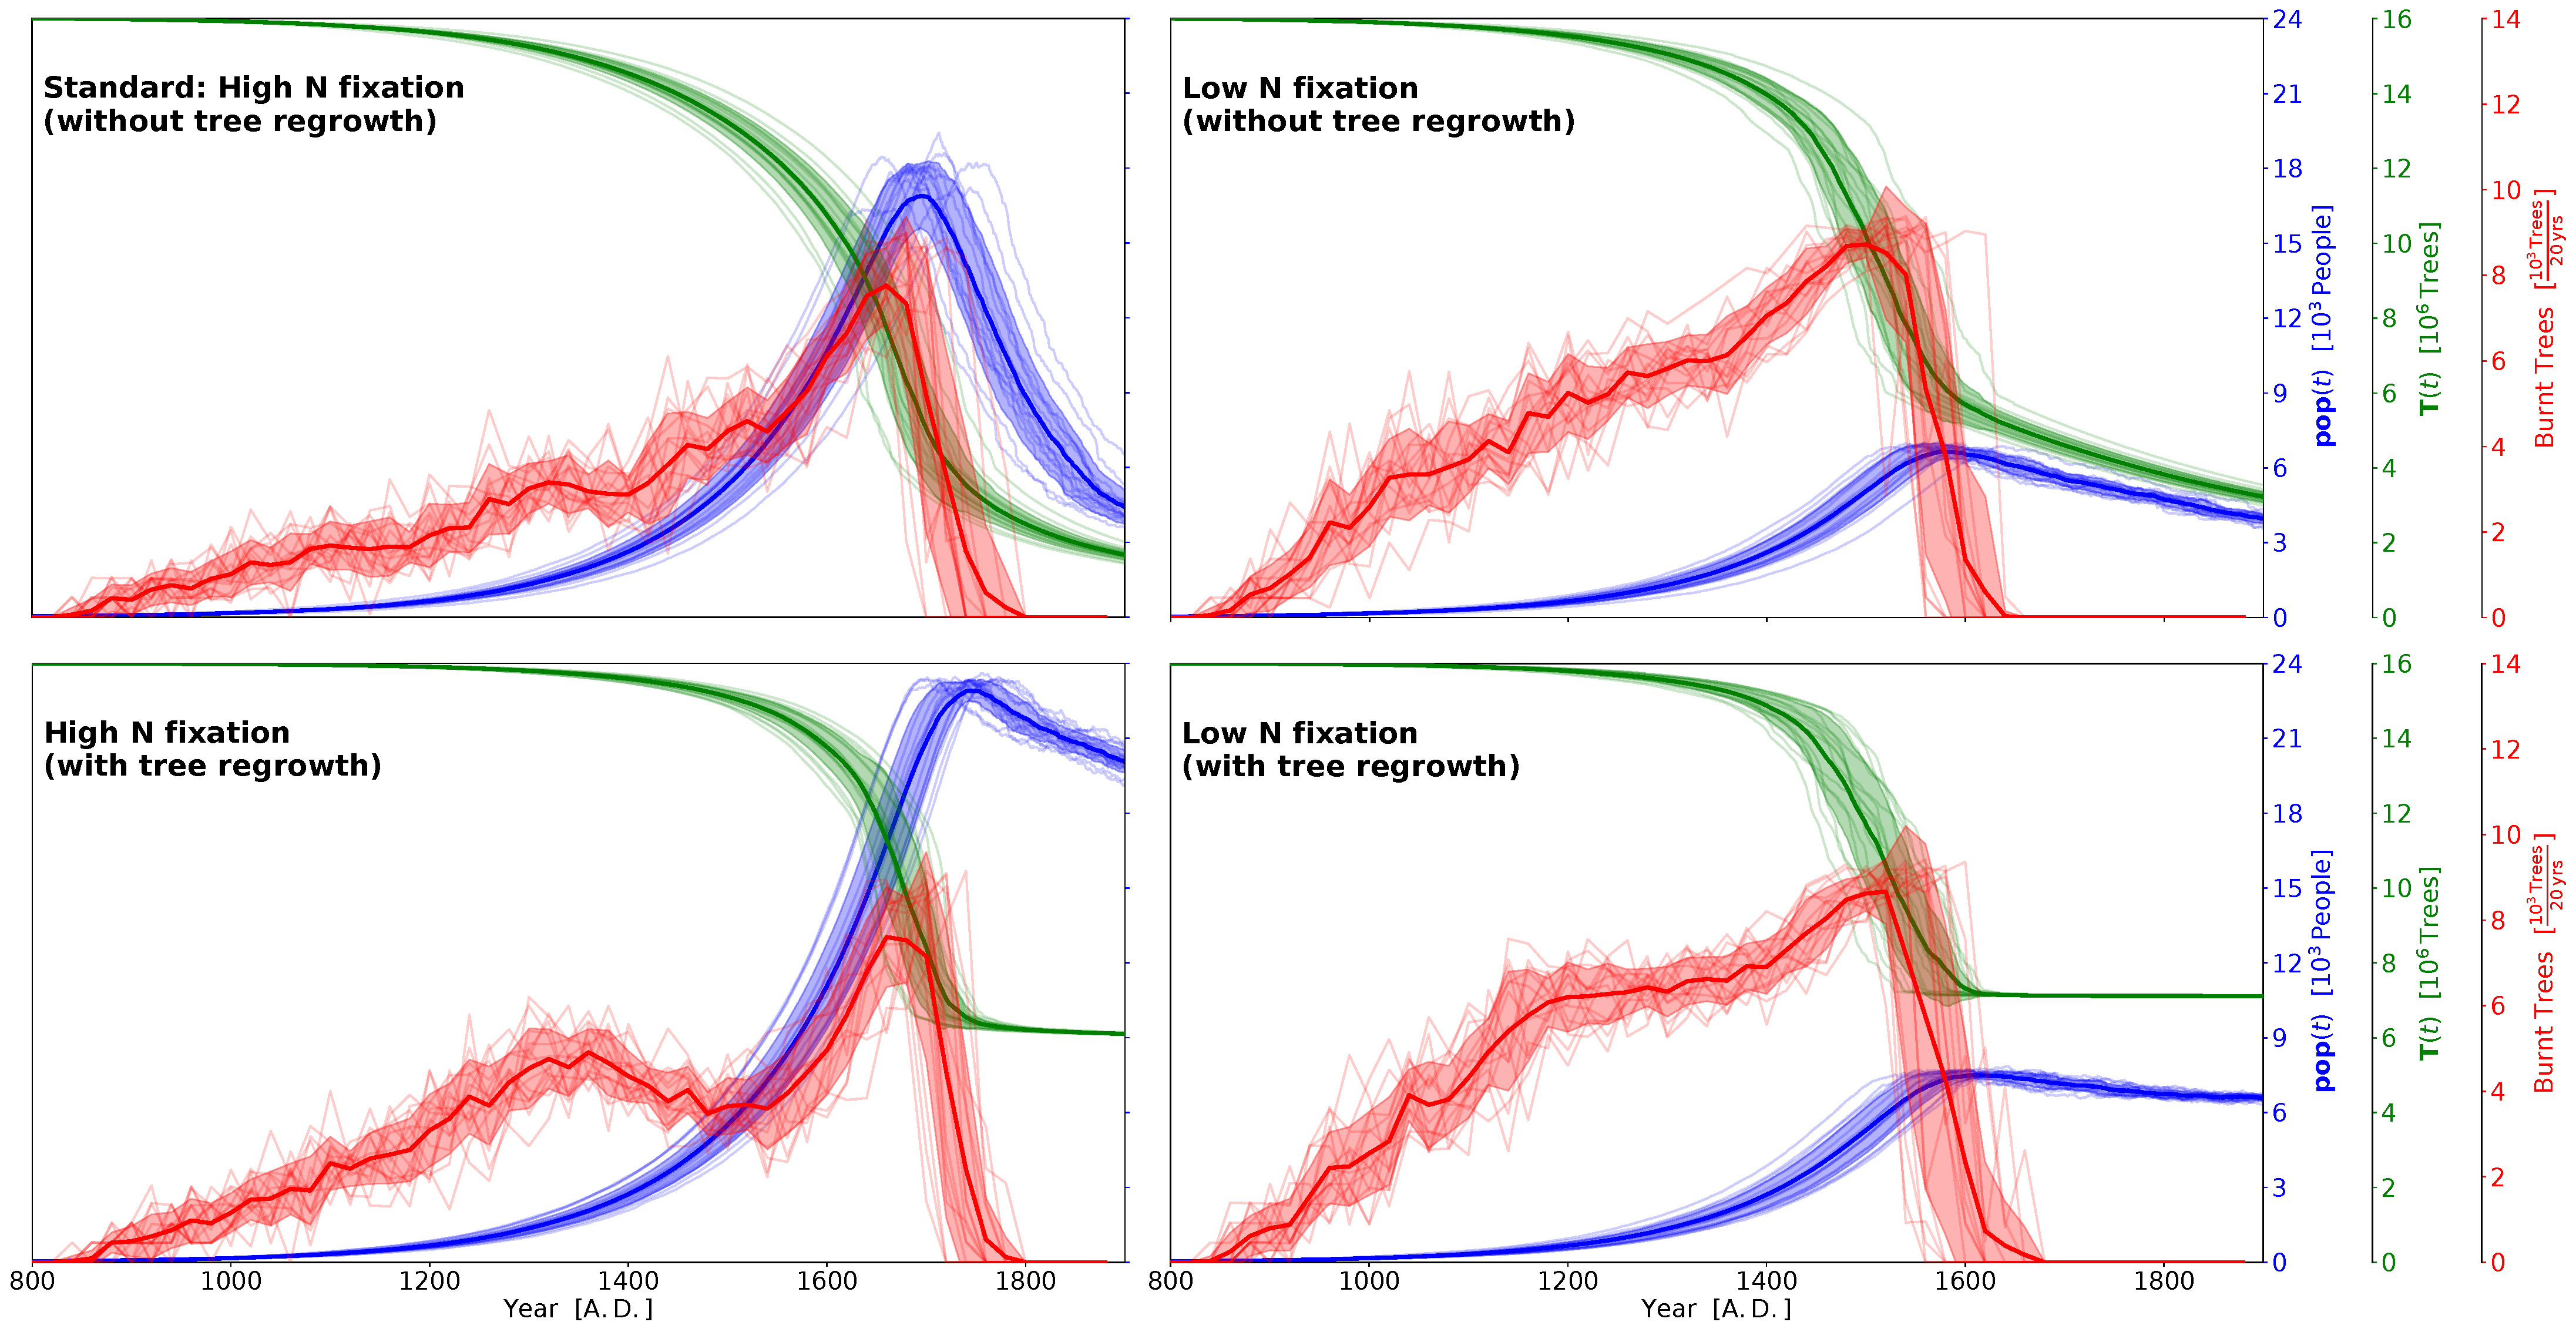
\includegraphics[width=1.3\textwidth, center]{images/Results/Standard/EnsembleStatistics_allTheories}
	\caption{Dynamics of aggregate population size, trees, and burnt trees for four different parameter settings: The high or low N fixation scenario determining the amount of arable land required per person in combination with disabled/enabled tree regrowth.
		All panels show mean dynamics obtained from an ensemble of 15 runs.}
	\label{fig:ensemblestatisticsalltheories}
\end{figure}

\subsection{Variation of the Resource Search Radii}
\begin{figure}
	\centering
	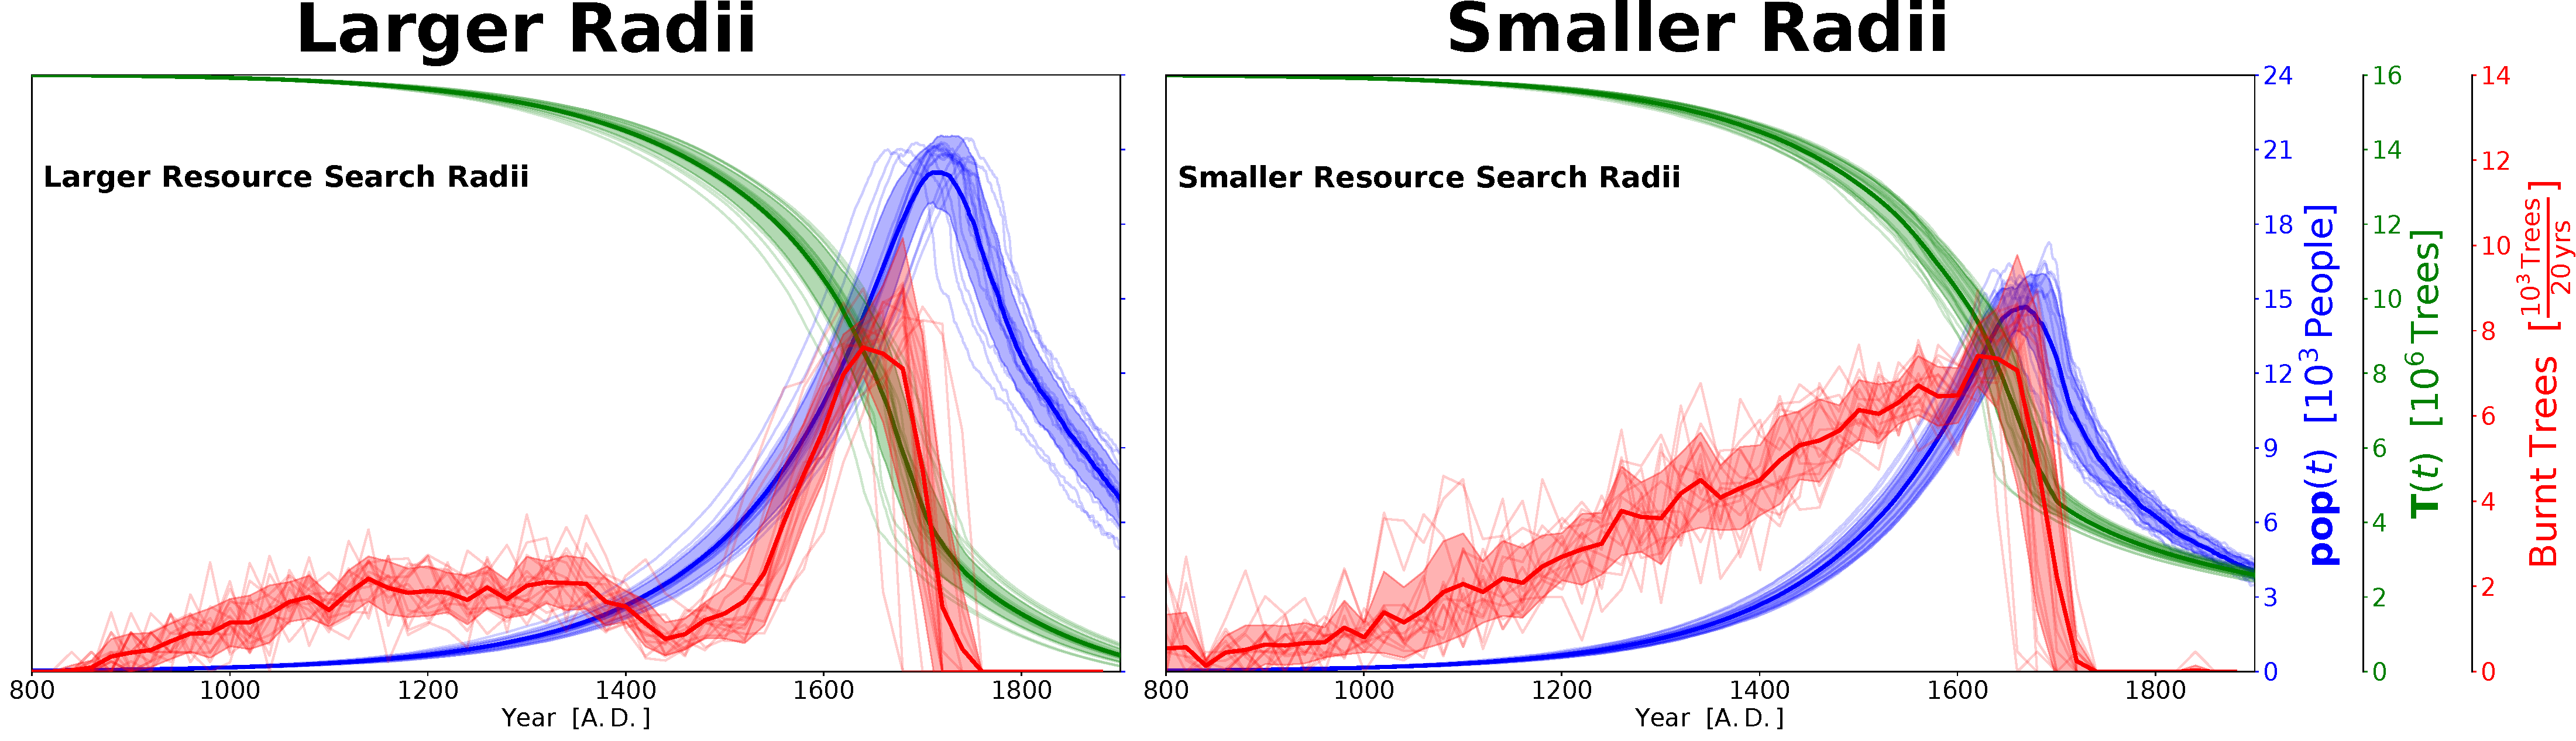
\includegraphics[width=1.3\linewidth, center]{images/Results/EnsembleStatistics_largersmallerRad}
	\caption{Dynamics of aggregate variables (as before) for variation of the resource search radii: The left panel shows runs with factor $2$ larger radii: $r_{\rm T}=4\, {\rm km}$ and $r_{\rm F}=2\, {\rm km}$; The right panel with factor $1/2$ smaller radii: $r_{\rm T}=1\, {\rm km}$ and $r_{\rm F}=0.5\, {\rm km}$. All variables strongly depend on the resource search radii which does not}
	\label{fig:ensemblestatisticslargersmallerrad}
\end{figure}

\paragraph{How the Resource Search Radii Change the Aggregate Dynamics.}
In Figure \ref{fig:ensemblestatisticslargersmallerrad}, I present a sensitivity analysis of the resource search radii which are in-/decreased by a factor of $2$ (left) or  $1/2$ (right) compared to the standard setting. 
For larger radius the peak population size increases, overall deforestation intensifies and the amount of burnt trees is low for a long time but rises steeply around $1600\, {\rm A.D.}$.
For smaller radius, the peak population size is strongly decreased, overall deforestation is smaller, and burning of trees increases linearly until a cut-off.
Variation of the resource search radius has a non-trivial influence on the aggregate dynamics.
On the one hand, a larger (or smaller) radius increases (or decreases, respectively) an agent's access to resources at its current location. 
On the other hand, it does not change the amount of available resources on the island, or required resources by agents.
As Figure \ref{fig:ensemblestatisticslargersmallerrad} shows, the differences of the results between those scenarios is significant. 
Even though the carrying capacity of the island with respect to the amount of resources is the same, the agent's harvest behaviour is restricted by its local context and, hence, this lack of either available arable land or trees in the local environment changes the shape of the aggregate dynamics in this model.

\paragraph{Caveat: Non-Existent Agent Cooperation.}
It is clear that the social and economic structure of the Easter Island population is much more complex than the independent, small households of a few dozen people acting independently and myopic assumed in this model. 
E.g.\ \citet{Diamond2011} describes the existence of roughly a dozen clans or chiefdoms, or \citet{Puleston2017} consider an economic structure including an elite and working class.
Also, there is clear evidence of exchange of goods between households and clans or chiefdoms, e.g.\ fish, stone tools or the Moai.
Such social structures would also allow for imposing taboos on the harvest of natural resources and increase the sustainability, as apparent on Easter Island \citep{Good2006}. 
All of theses complex, cooperative structures based on agent-agent interactions are not considered here, but each agent farms and deforests individually.
Including such political institutions would decrease the influence of the local confinement on the population dynamics.

\paragraph{Outlook: Clusters and Chiefdoms.}
The model presented here can be extended to show the emergence of clustered agents that cooperatively harvest resources.
E.g.\ Figure \ref{fig:clusterstds1650} shows the centre points of $7$ clusters obtained by k-Means clustering of the three dimensional space spanned by the agent's position and tree preference trait, $\left( x_{\rm i}, y_{\rm i}, T_\text{Pref, i} \right)(t)$ for agent $i$, in one specific year, $1650\, {\rm A.D.}$ using the python packages \textit{scikit-learn}\footnote{\citet{scikit-learn}} and \textit{yellowbrick}\footnote{\citet{yellowbrick}}.
For all tested years (between $1200$ and $1900\, {\rm A.D.}$) a number of $7$ to $9$ clusters are optimal according to the elbow method\footnote{The elbow is a heuristic to estimate the number of clusters:
	Running the k-Means algorithm with more clusters only linearly decreases the distortion, i.e.\ the sum of the squared distances of an agents 3D state to the cluster centres.}.
While this analysis is very preliminary, clustering might open the possibility of including stronger links within clusters of agents, that tend to move towards each other (e.g.\ negative population density penalty), harvest cooperatively, and increase the resource search radius with the cluster size.
One could even think of a trading module between clusters (as in \citen{Heckbert2013}).
Future research with this model could investigate more complex economic and social structures and, thereby, overcome one of the major weakness, the self-centred, non-cooperative harvest behaviour of agents.

\FloatBarrier
\subsection{Variation in the Population Growth Module}

\paragraph{Impact on the Aggregate Dynamics.}
I test the stability of the model results to a less resilient demography model.
By increasing the shape parameter of $g(H_{\rm i})(t)$ an agent's population size declines steeper and earlier as $H_{\rm i}(t)$ drops.
%and, thereby, increasing the required happiness to remain at a constant population size, $H_{\rm euq}$ a population decline sets in earlier and more extreme in most cases.
However, in the standard run, happiness of the agents decreases rapidly from $1$ to $0$ typically close to the peak population size and an agent can not find a place sufficient for meeting both resource requirements.
Hence, the results are nearly indifferent to this variation of the population growth model\footnote{In this simulation the ensemble net population decrease sets in only $10$ years prior to the standard case and at the same peak level.}.
However, for the scenario with tree regrowth 
the stable equilibrium between tree regrowth and tree cutting can sustain fewer individuals (roughly $2000$, not shown) for this less resilient population scenario and its higher equilibrium happiness, $H_{\rm equ}$.
%decreases the population size in the stable equilibrium (and the peak) by roughly $2000$ individuals (not shown).

\paragraph{Caveat: Oversimplified Population Growth Module.}
The population dynamics in this ABM is subject to several limitations.
The use of the food-limited demography model from \citet{Puleston2017} is strongly simplified here.
E.g.\ I use a different notion of \citet{Puleston2017}'s food ratio, which I express via the smoothed happiness $H_\text{i}(t)$ reflecting the success in cutting trees and farming.
Also the distinction between survival and fertility rate especially given their age-dependency is entirely neglected.
One major problem with the assumed population dynamics in this model is the fast decrease of effective happiness when the resource, trees, is missing and the agent can not find a place on the island sufficient to sustain it with both trees and farming produce simultaneously and, therefore, perishes quickly.
Another issue is the unabated exponential growth of the population independent of population density.
%Therefore, in the model agents quickly vanish as local resource scarcity sets in and suitable spots that fill both resource requirements are not available anymore.
The model would greatly benefit from a smarter, more dynamic integration of the demography model by \citet{Puleston2017} and, in general, a more advanced relation between the tree and farming harvest and the population growth in this model.


\subsection{Variation of the Strategy of Adapting the Tree Preference}
%\paragraph{Differences in Burnt Trees, Population Size and Deforestation given the different adaption speed of the tree preference to local environmental changes}
%\begin{itemize}
%	\item Runs with $f_{\rm Tree \ Pref}$ delayed, careful, logistic.
%\end{itemize}

%\paragraph{Impacts on the Aggregate Dynamics of Different Adaption Strategies}
The change of the tree preference in response to local deforestation is the only far-sighted adaption mechanism of the agents in the harvest process in response to the environmental degradation.
In the standard setting, an agent's tree preference responds linearly to the removal of trees.
In Section \ref{sec:agentprops}, I presented three alternative adaption strategies: Delayed, faster (i.e.\ with foresight), and logistic adaption (first delayed, then faster) (see Figure \ref{fig:TPref_T}).
\begin{figure}
	\centering
	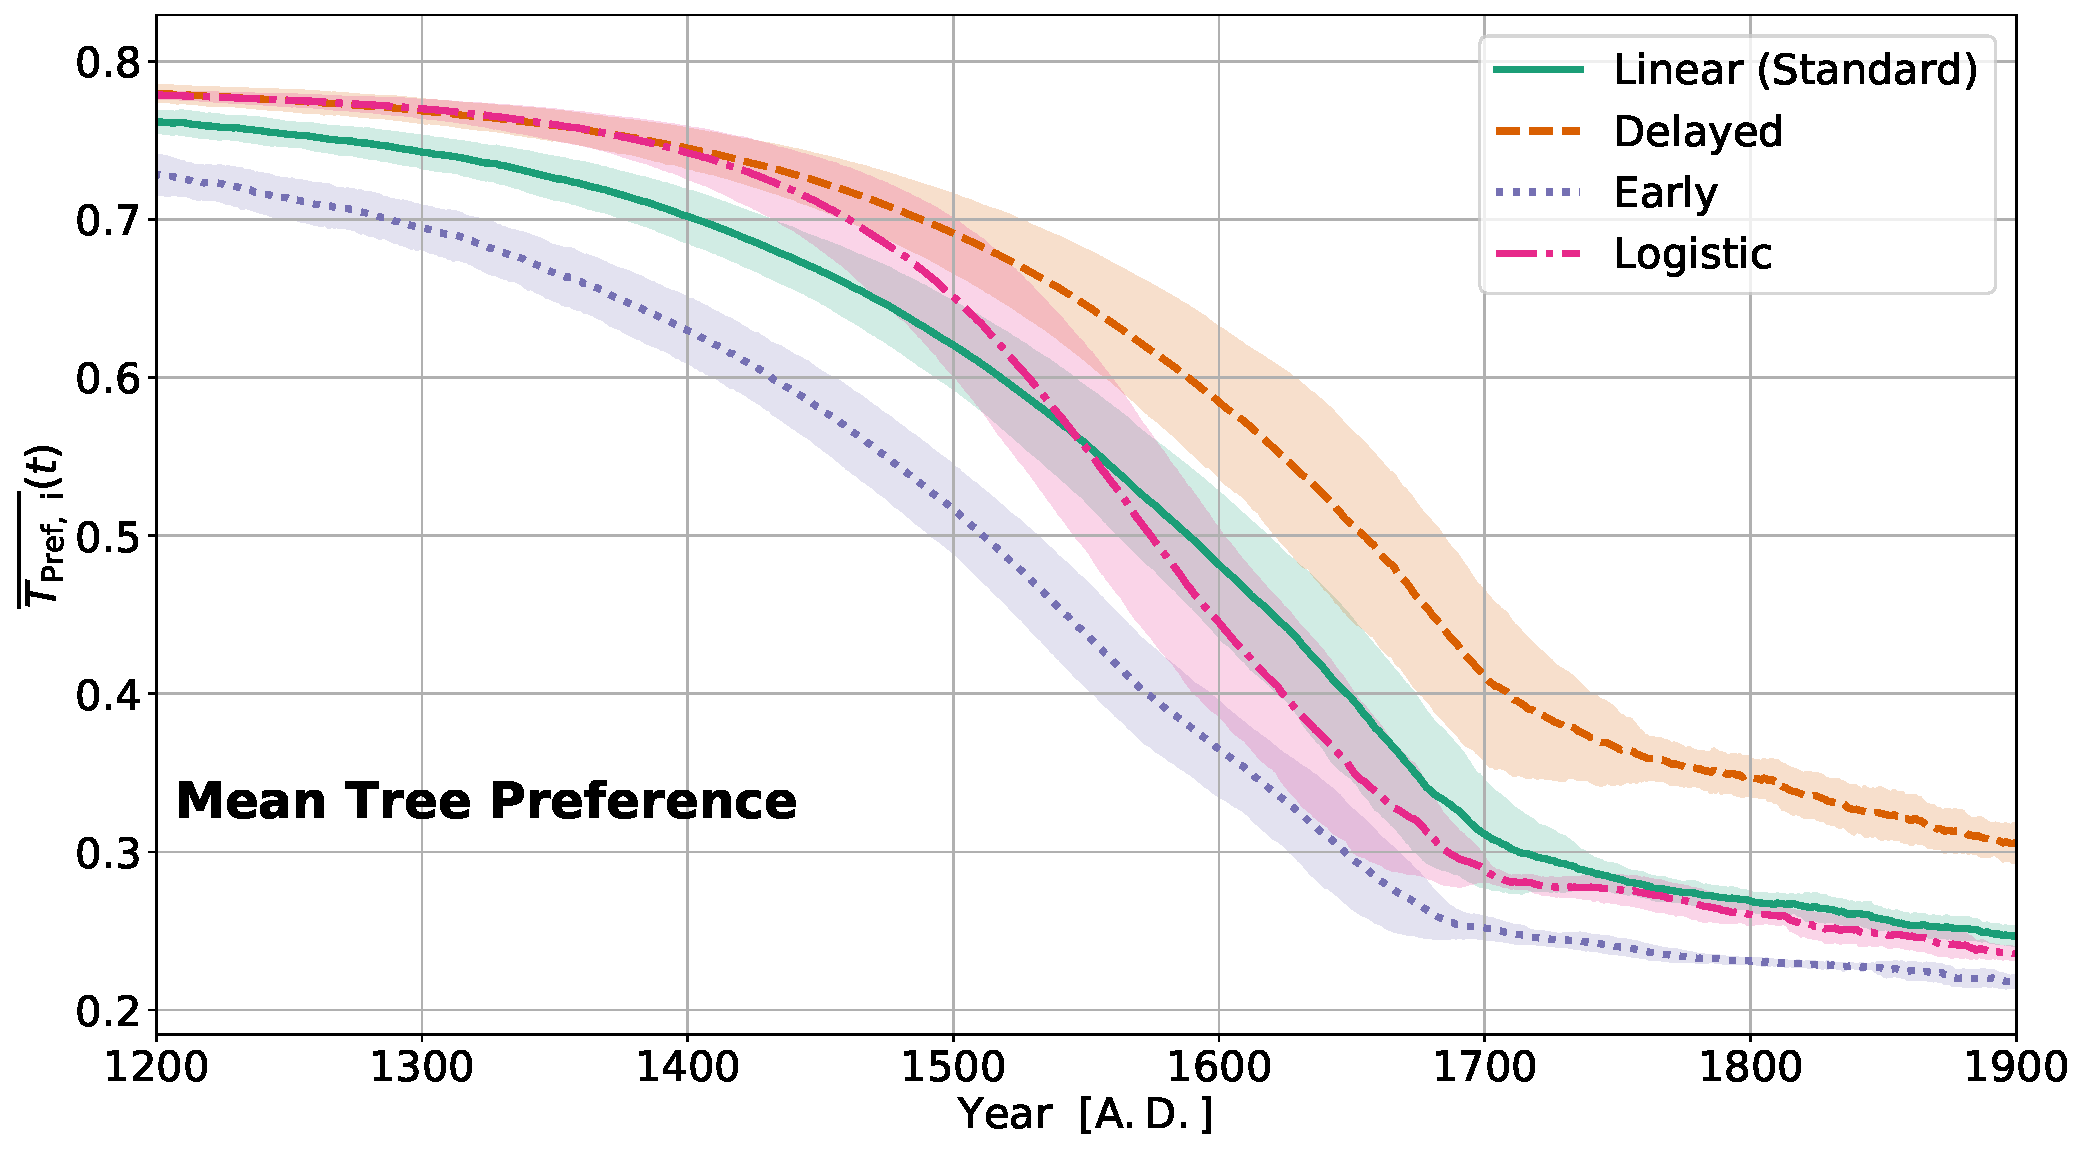
\includegraphics[width=1\linewidth]{images/Results/TPref/TPrefAdaption_TPref}
	\caption{Mean tree preferences of all agents $\overline{T_\text{Pref, i}(t)}$ over time from an ensemble of each 15 different model realisations with different strategies to adapt the tree preference to the changing local tree density: Linear (standard setting), delayed, faster, or logistic (all shown in Figure \ref{fig:TPref_T}).}
	\label{fig:tprefadaptiontpref}
\end{figure}
The mean tree preference of all agents, $\overline{T_\text{Pref, i}(t)}$, is shown in Figure \ref{fig:tprefadaptiontpref} for an ensemble of 15 realisations each.
%As expected the mean tree preference decreases delayed in the delayed, faster in the faster adaption scenario and in between for the linear and logistic adaption scenarios. 
%This, however, has non-linear consequences for the society described in the following.
The corresponding population dynamics is shown in Figure \ref{fig:tprefadaptionpopulationsize}.
%The population of the logistic case peaks earliest (at a lower level as the peaks of )and also declines faster than the others. 
The population size in the fast adaption scenario peaks at a high value (and later) than with other strategies.
The logistic strategy first follows the curve of the  delayed strategy, but then converges to the linear, standard strategy.
Eventually, the population size (in $1900\, {\rm A.D.}$) is nearly twice as high for a fast vs.\ delayed adopting society.
%In the, in the year $1900$ of the simulation, $6000$ people remain in the faster adaption scenario compared to ca. $4000$ in the logistic or delayed adaption scenarios.
Similarly, the dynamics of the deforestation level (Figure \ref{fig:tprefadaptiontrees}) and burnt trees (Figure \ref{fig:tprefadaptionburnttrees}) depend on the tree preference adaption strategy. 
If tree preference is adopted fast, fires increase continuously from beginning to the peak. 
Especially with delayed and logistic adoption, the amount of trees burnt stagnates (or even decreases) between $1300$ and $1500\,{\rm A.D.}$ followed by a sharp increase afterwards.
The summed amount of burnt trees is highest in the faster adoption in the faster ($5.3\cdot 10^6$), compared to linear ($4.3\cdot 10^6$), logistic ($4.4\cdot 10^6$) and delayed ($3.3\cdot 10^6$) strategy.
Still, counter-intuitively in total more trees remain at the end of the simulations with fast adaption.
The mean happiness of all agents is also slightly higher (or equivalent) for the fast adoption strategy throughout the time period (not shown).
In summary, the specific shape of the adaption of the tree preference to local environmental change has a non-trivial influence on the aggregate dynamics.

The results show that, in summary, a fast decrease (or early adaption) of the tree preference seems to be the best strategy for the agents in all aspects, maximising the peak and final population size, the amount of trees, and the mean happiness.
While the logistic and linear strategies are quite similar in their aggregate outcomes, the peak population size is smaller for the logistic strategy.
Hence, it seems that a better strategy for a civilisation in this model is to adapt linearly early to local tree density changes rather than later but then  with a steeper adaption speed (as in the logistic strategy) to `catch up'.

\begin{figure}
	\centering
	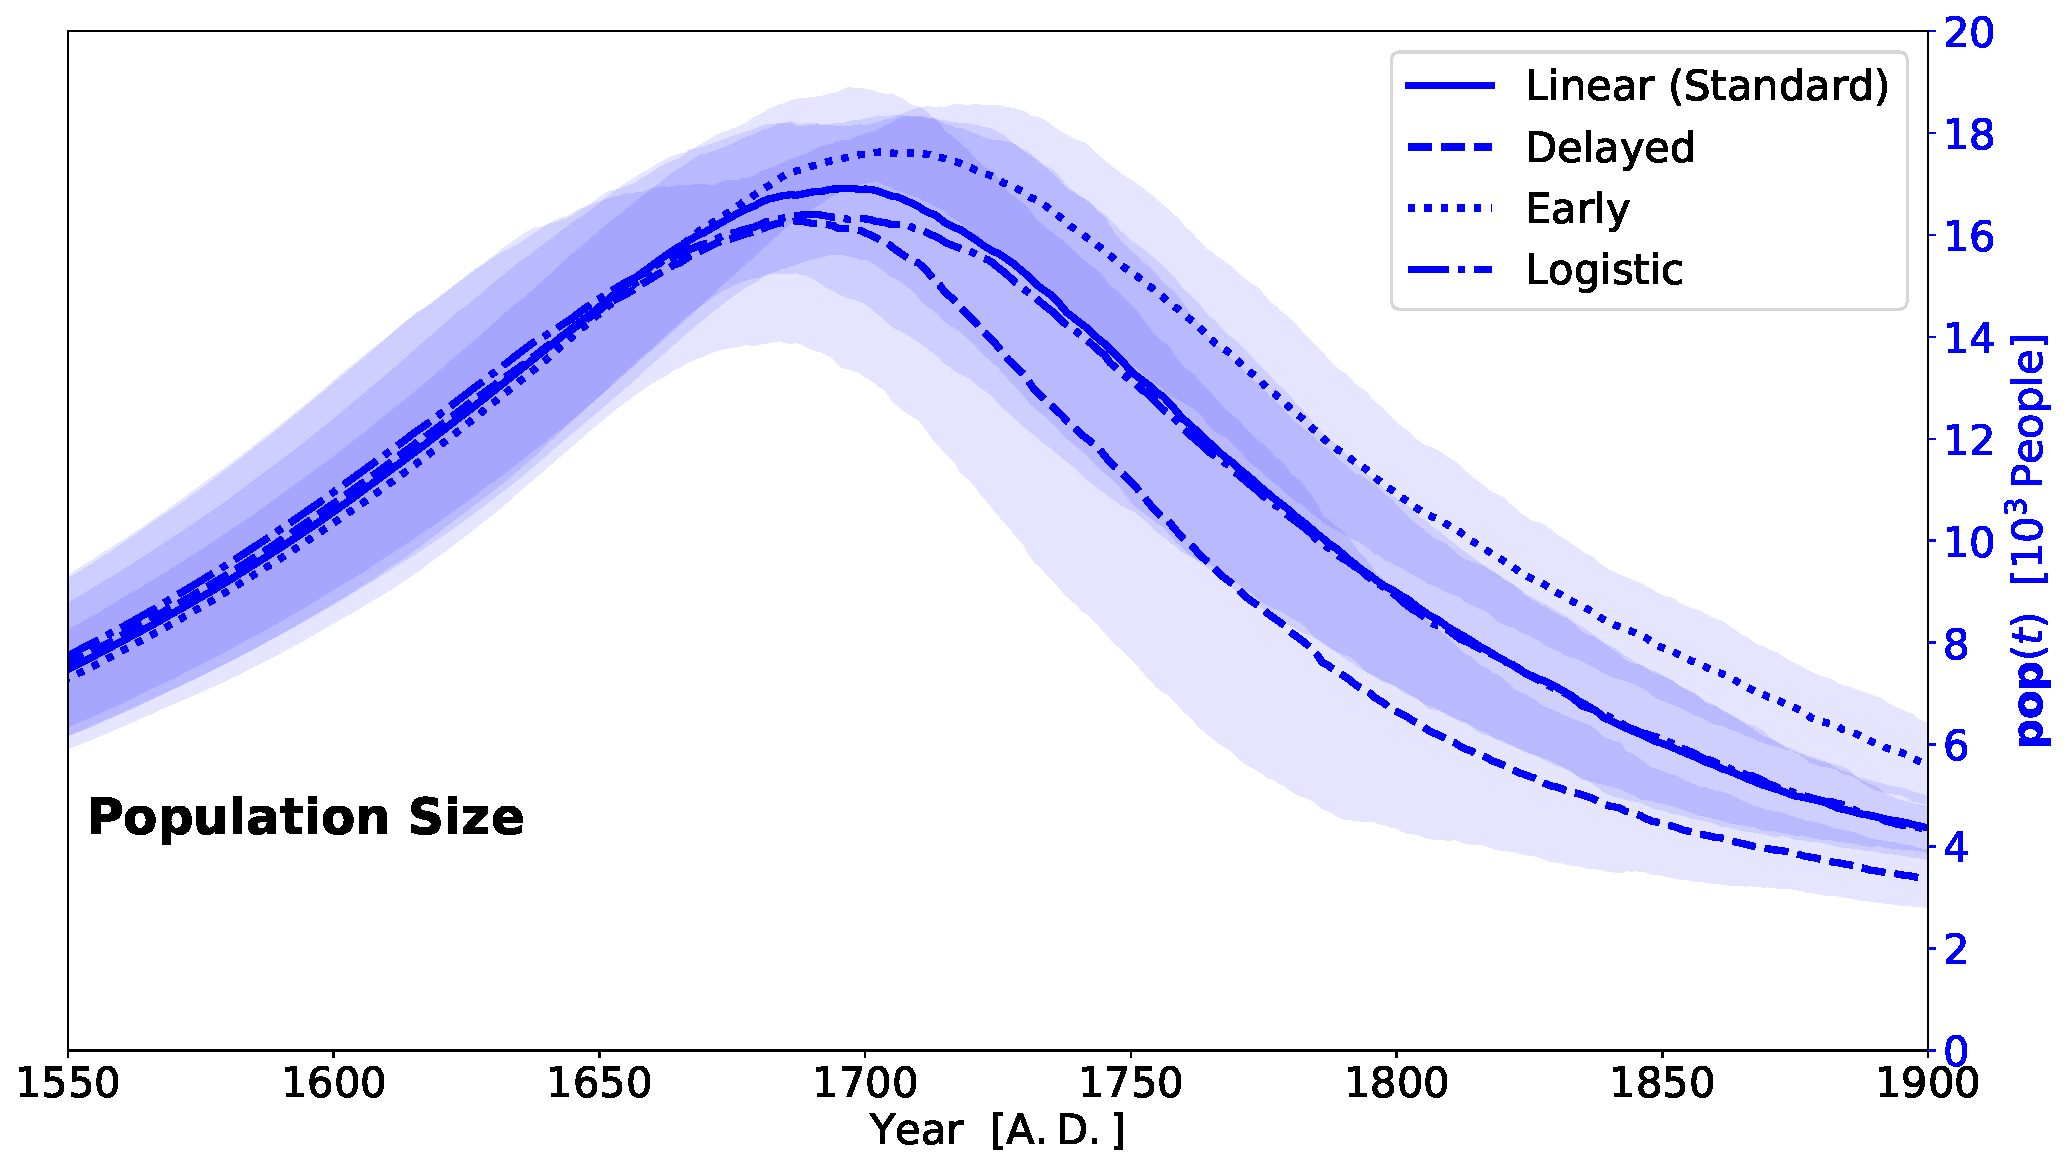
\includegraphics[width=1\linewidth]{images/Results/TPref/TPrefAdaption_Population_Size}
	\caption{Total aggregate population dynamics for the different adaption strategies in relation to the tree preference.}
	\label{fig:tprefadaptionpopulationsize}
\end{figure}




%
%The happiness decreases quite similar in all four adoption strategies. However, early in the phase of population decrease, the 
%(Figure \ref{fig:tprefadaptionhappy})
%
% and the mean happiness of all agents, $\overline{h_{\rm i}(t)}$ in Figure \ref{fig:tprefadaptionhappy}.
%\begin{figure}
%	\centering
%	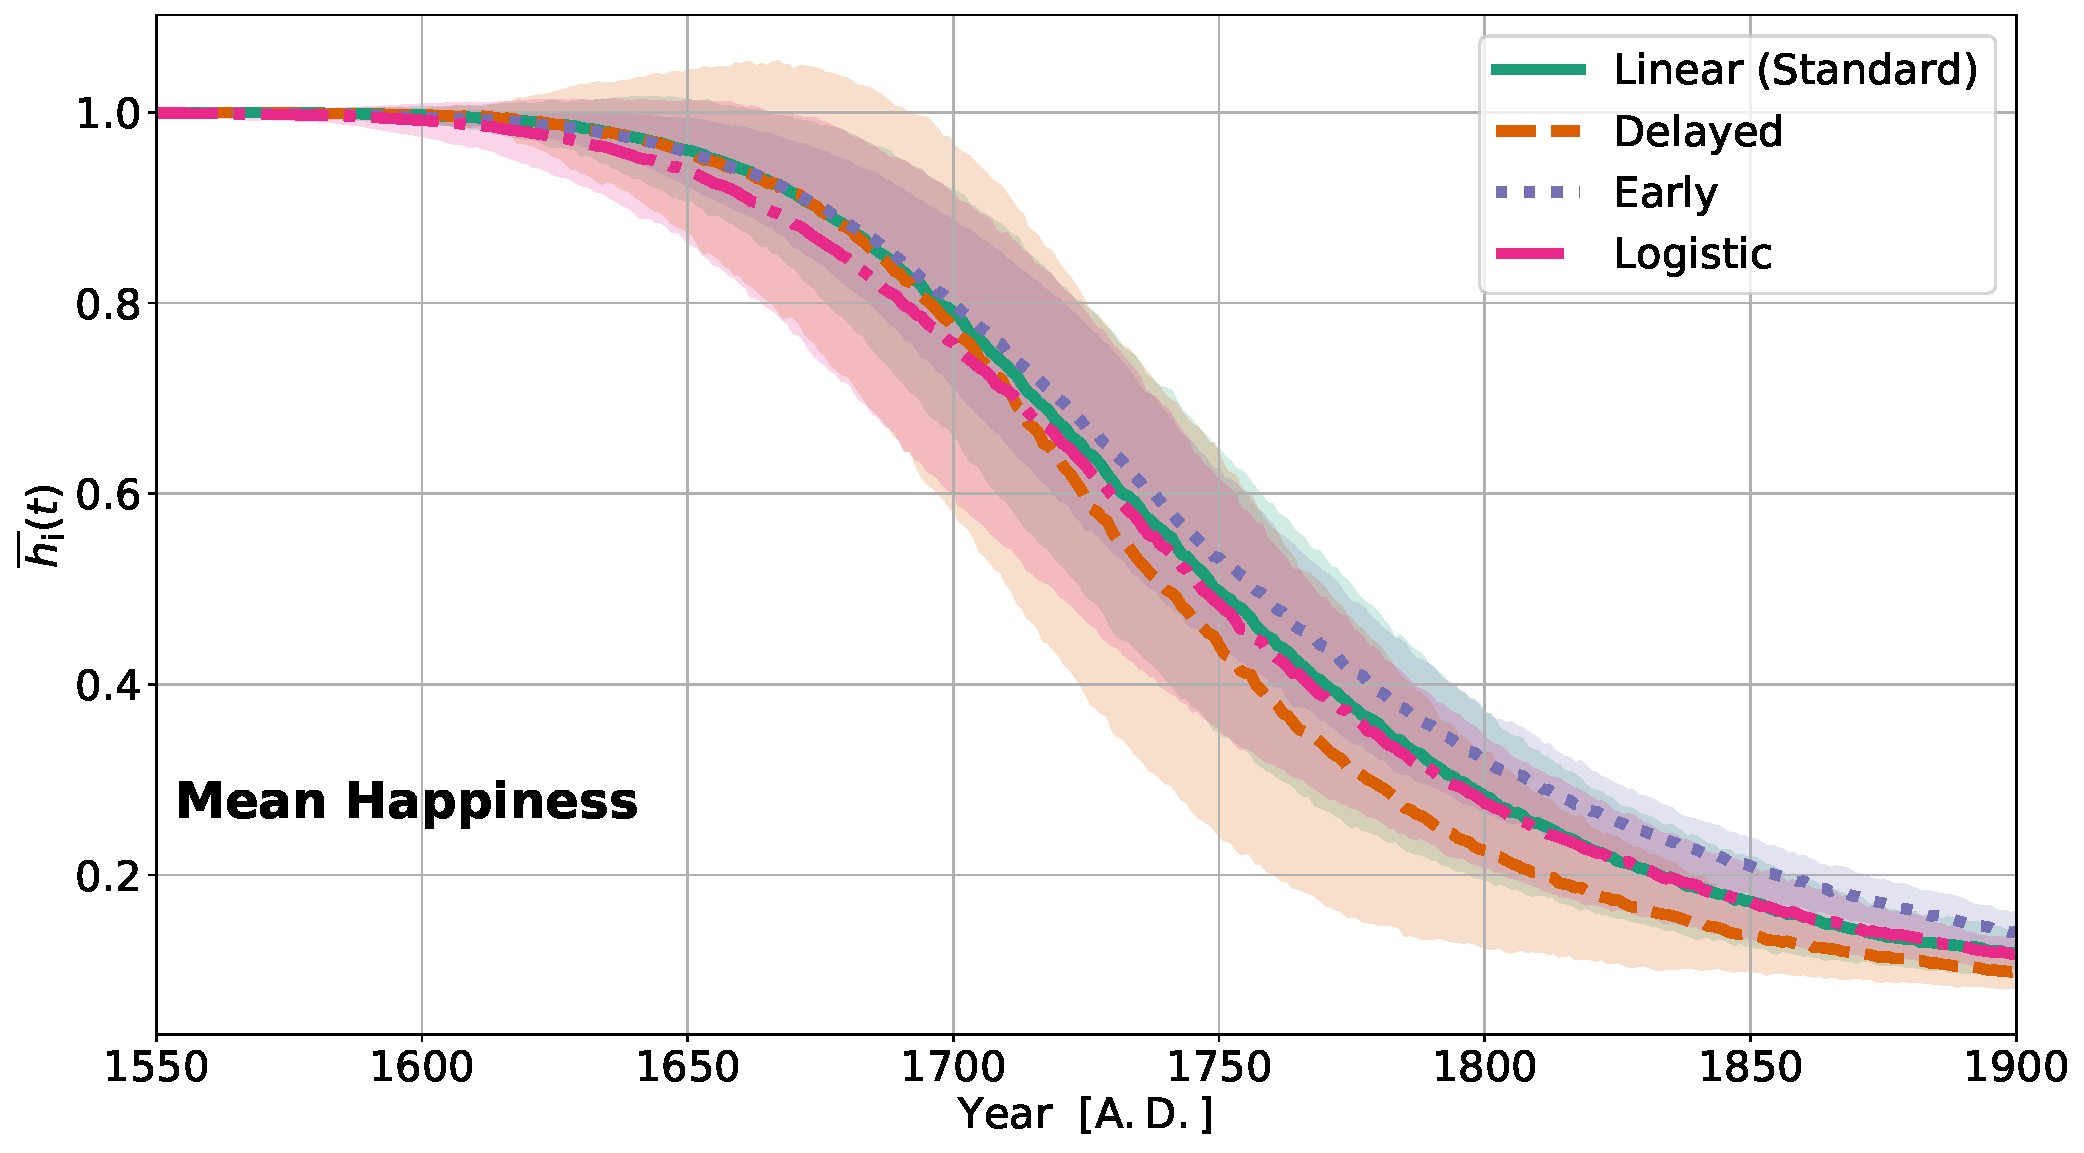
\includegraphics[width=1.0\linewidth]{images/Results/TPref/TPrefAdaption_Happy}
%	\caption{Ensemble mean of the mean happiness of all agents $\overline{T_\text{Pref, i}(t)}$ over time from five different model realisations with the different tree preference adaption strategies as previously described in Figures \ref{fig:tprefadaptiontpref} and \ref{fig:tprefadaptionpopulationsize}}.
%	\label{fig:tprefadaptionhappy}
%\end{figure}



%\section{Variation of some uncertain parameters}
%$r_{\rm T}$, $r_{\rm F}$,
%$T_{\rm Req, pP}$


\subsection{Variation of the Decision Making Strategy in the Moving Module}
%\paragraph{Description of differences obtained when the decision making is (1) based on penalties and (1a) stochastic, (1b) deterministic, (1c) only based on resource availability or decision making is (2) entirely random.}
%\begin{itemize}
%	\item Standard setting, $\gamma=20$, $\alpha=(0.2,0.2,0.2,0.2,0.2)$.
%	\item `Only resource availability matters for moving decision' setting, $\gamma=20$, $\alpha=(0, 0, 0, 0.5,0.5)$.
%	\item Hopping agents, that move to a random spot with uniform probability over the island, $\gamma=0$, $\alpha=$ doesn't matter.
%\end{itemize}
%Results not yet known. I guess I'll describe qualitatively what happens to the spatial patterns. 
%If the aggregate dynamics change, this would of course be a big, big result and I would focus on that.

\paragraph{Moving Strategies and their Impacts on the Spatial and Aggregate Dynamics.}
In the analysis so far, I have distinguished between spatial patterns on the one hand and the aggregate dynamics on the other.
However, the results in this Section show that the spatial patterns also have an influence on the aggregate variables, population size and number of trees and burnt trees.
Here, I investigate how three different decision making strategies in the moving module (see also Table \ref{tab:sensitivity}) compare with the standard setting described above. The strategies consider
\begin{itemize}
	\item  all penalties equally high, including some stochasticity (the standard run, as described in Figure \ref{fig:STDrull}) 
	\item `only resource' penalties (Figure \ref{fig:resource}), i.e. $\alpha_{\rm T}= \alpha_{\rm F} = 0.5$ and all other weights are zero.
	Here, agents spread out on all locations with access to arable, well-suited land irrespective of distance from freshwater, elevation, slope and population density.
	Consequently, the amount of trees burnt is larger in the period from $1200$ to $1600\, {\rm A.D.}$ as there are no dense population centres in which collective tree cutting contributes to the clearing of land. 
	Population peaks at a slightly later time and at a higher level. 
	The following population size decrease after the peak is steeper and less individuals remain in $1900\, {\rm A.D.}$.
	\item only the `optimal location' with the smallest penalty, i.e.\ a fully deterministic moving decision with $\gamma>>1$ and $\vec{\alpha}$ as in the standard setting (Figure \ref{fig:optimal}).
	Interestingly, agents cluster around `highly evaluated' spots leading to a patchy spatial pattern. The aggregated population size (including the peak level), number of burnt trees or tree number are mostly unaffected by this, though, in comparison to the standard run but the variation in peak population size is smaller.
	\item no penalties or evaluation criteria at all, i.e.\ agents ignore all penalties ($\gamma = 0$) and perform a `Trial\&Error Hopping' (Figure \ref{fig:hop}).
	Hence, an agent might `hop' around in consecutive years until a spot with sufficient resource access is found, but burn trees to set up farms that are abandoned soon after throughout this search.
	This process delays the population growth, and, consequently, the population size peaks a century later (shortly before $1800\, {\rm A.D.}$) but at a similar peak size compared to the standard run. The peak population is followed by a rapid decline (up to $2\%$ per year) to a third of the population size within less than a century.
\end{itemize}
\begin{figure}
	\centering
	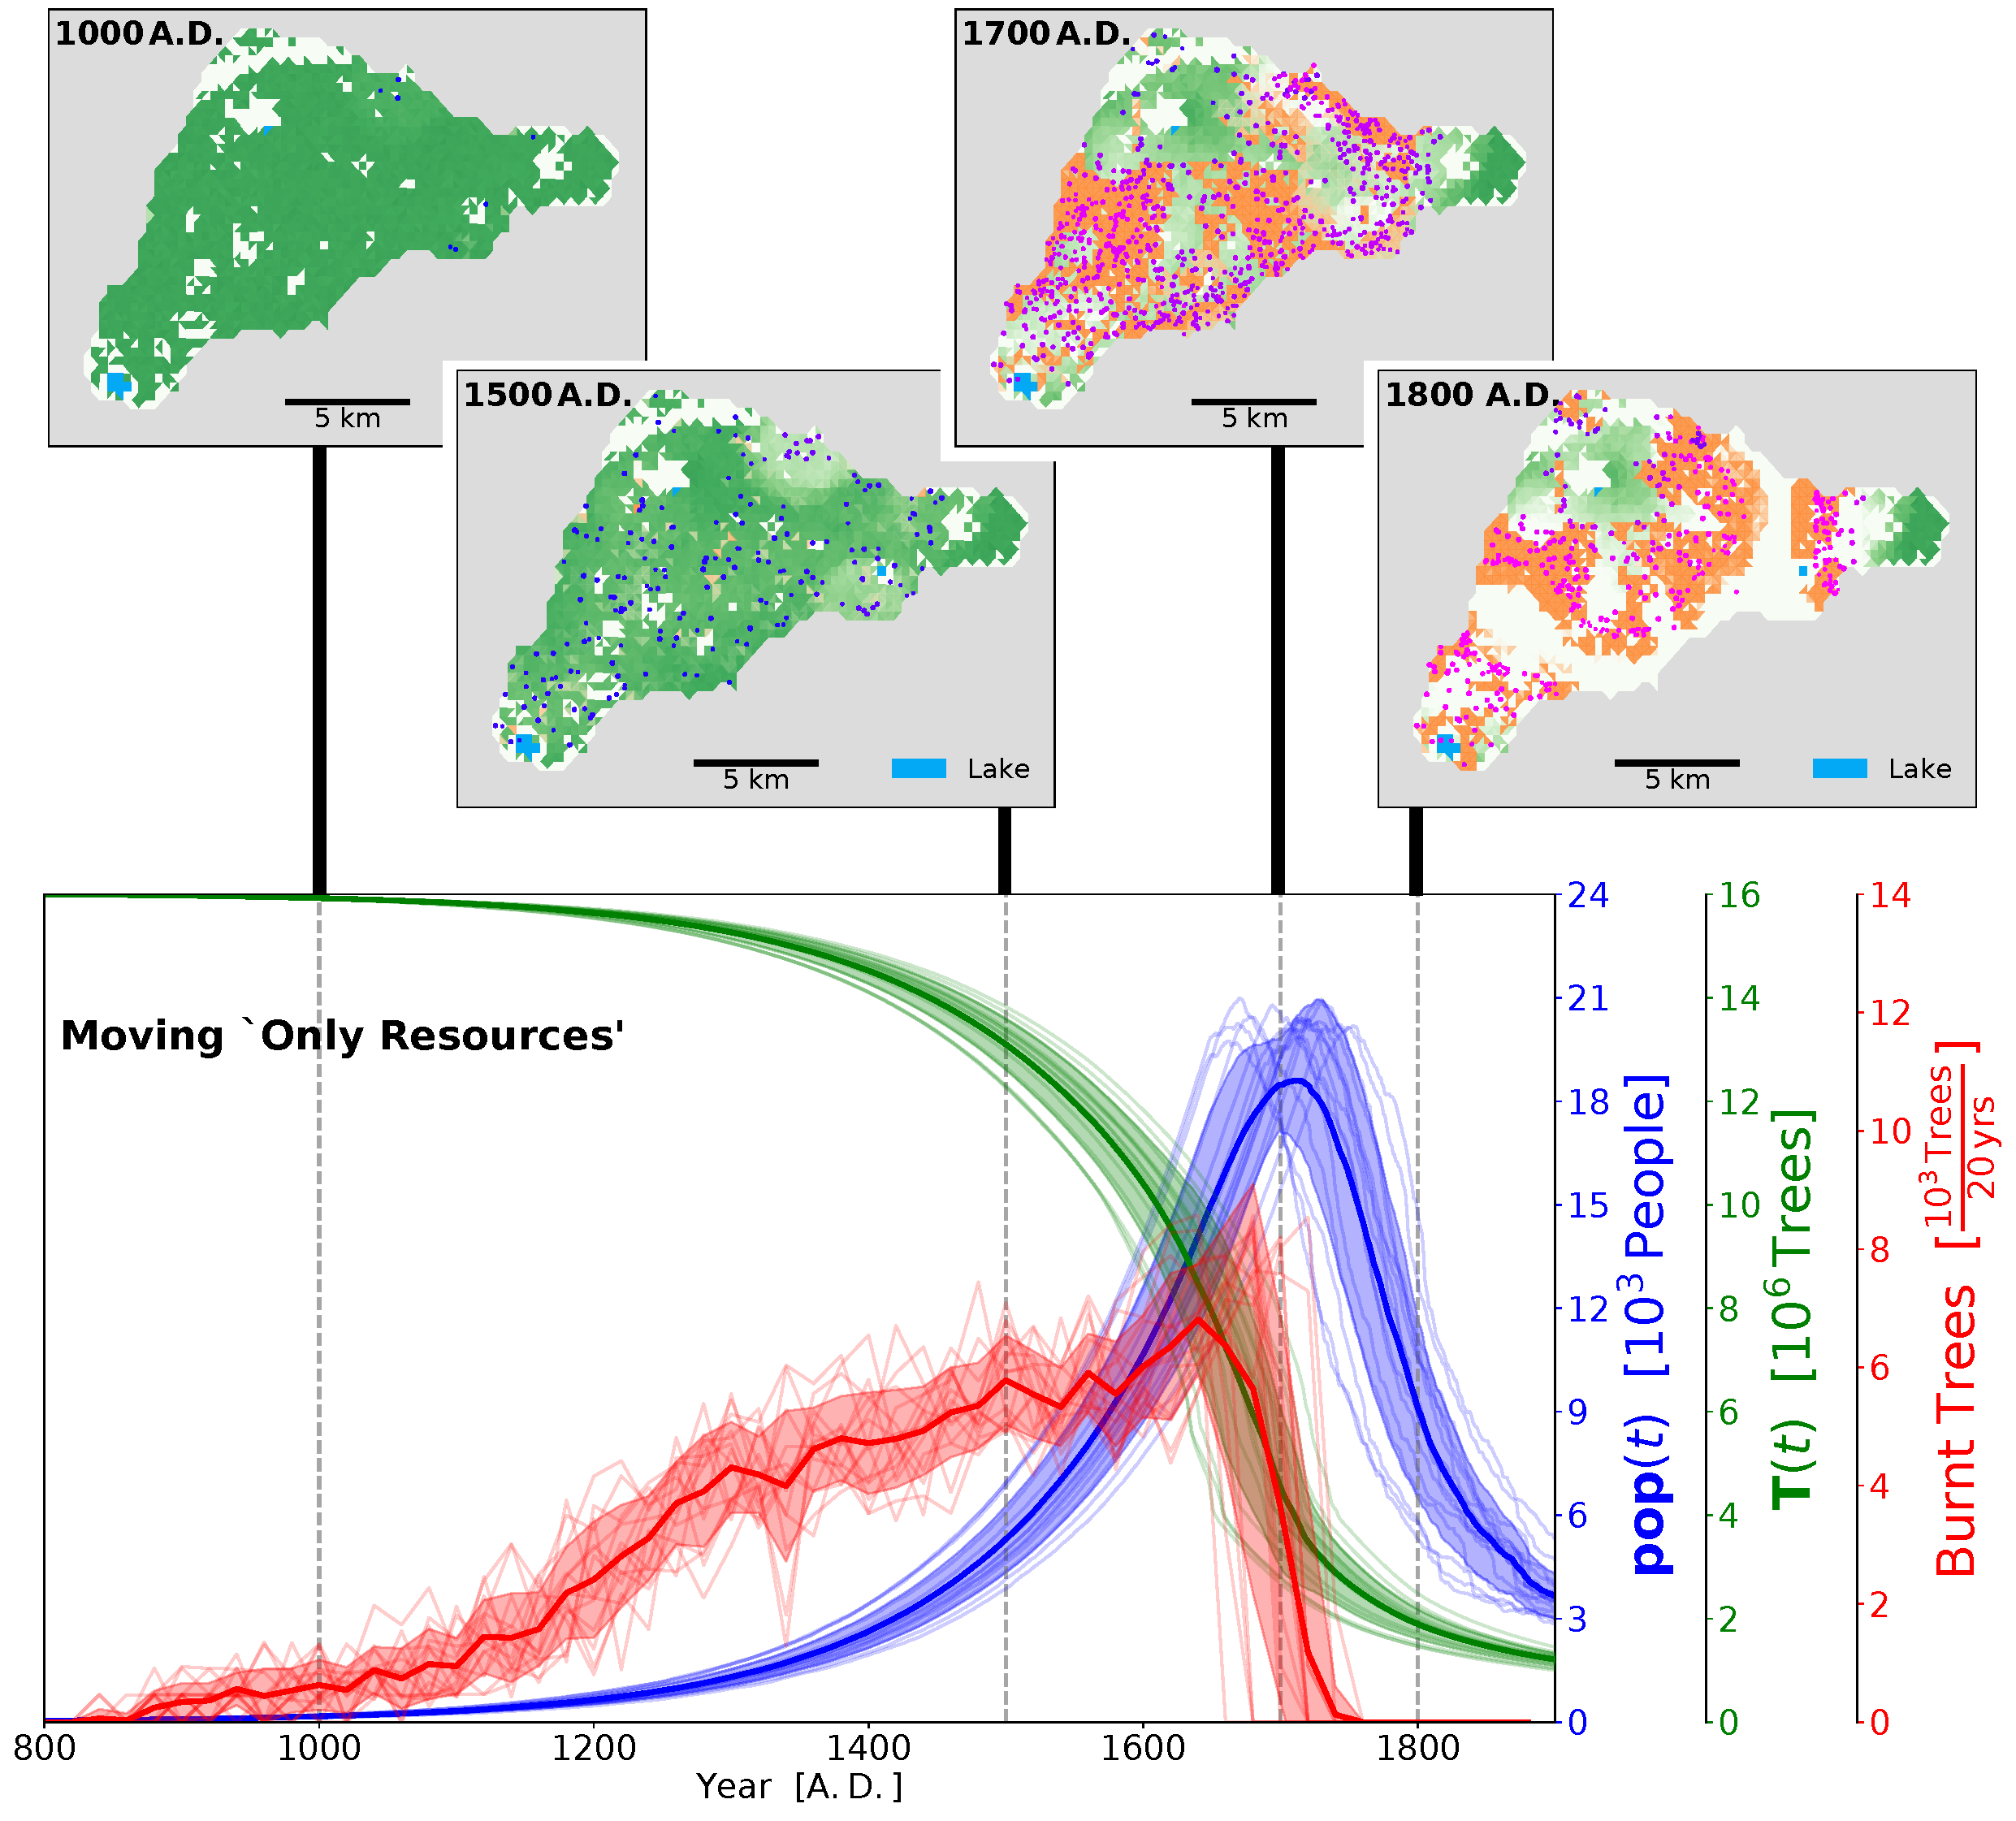
\includegraphics[width=1\textwidth]{images/Results/Moving/alphaResource_EnsembleStatistics+Panels}
	\caption{Moving strategy `Only Resources'.}
	\label{fig:resource}
\end{figure}
\begin{figure}
	\centering
	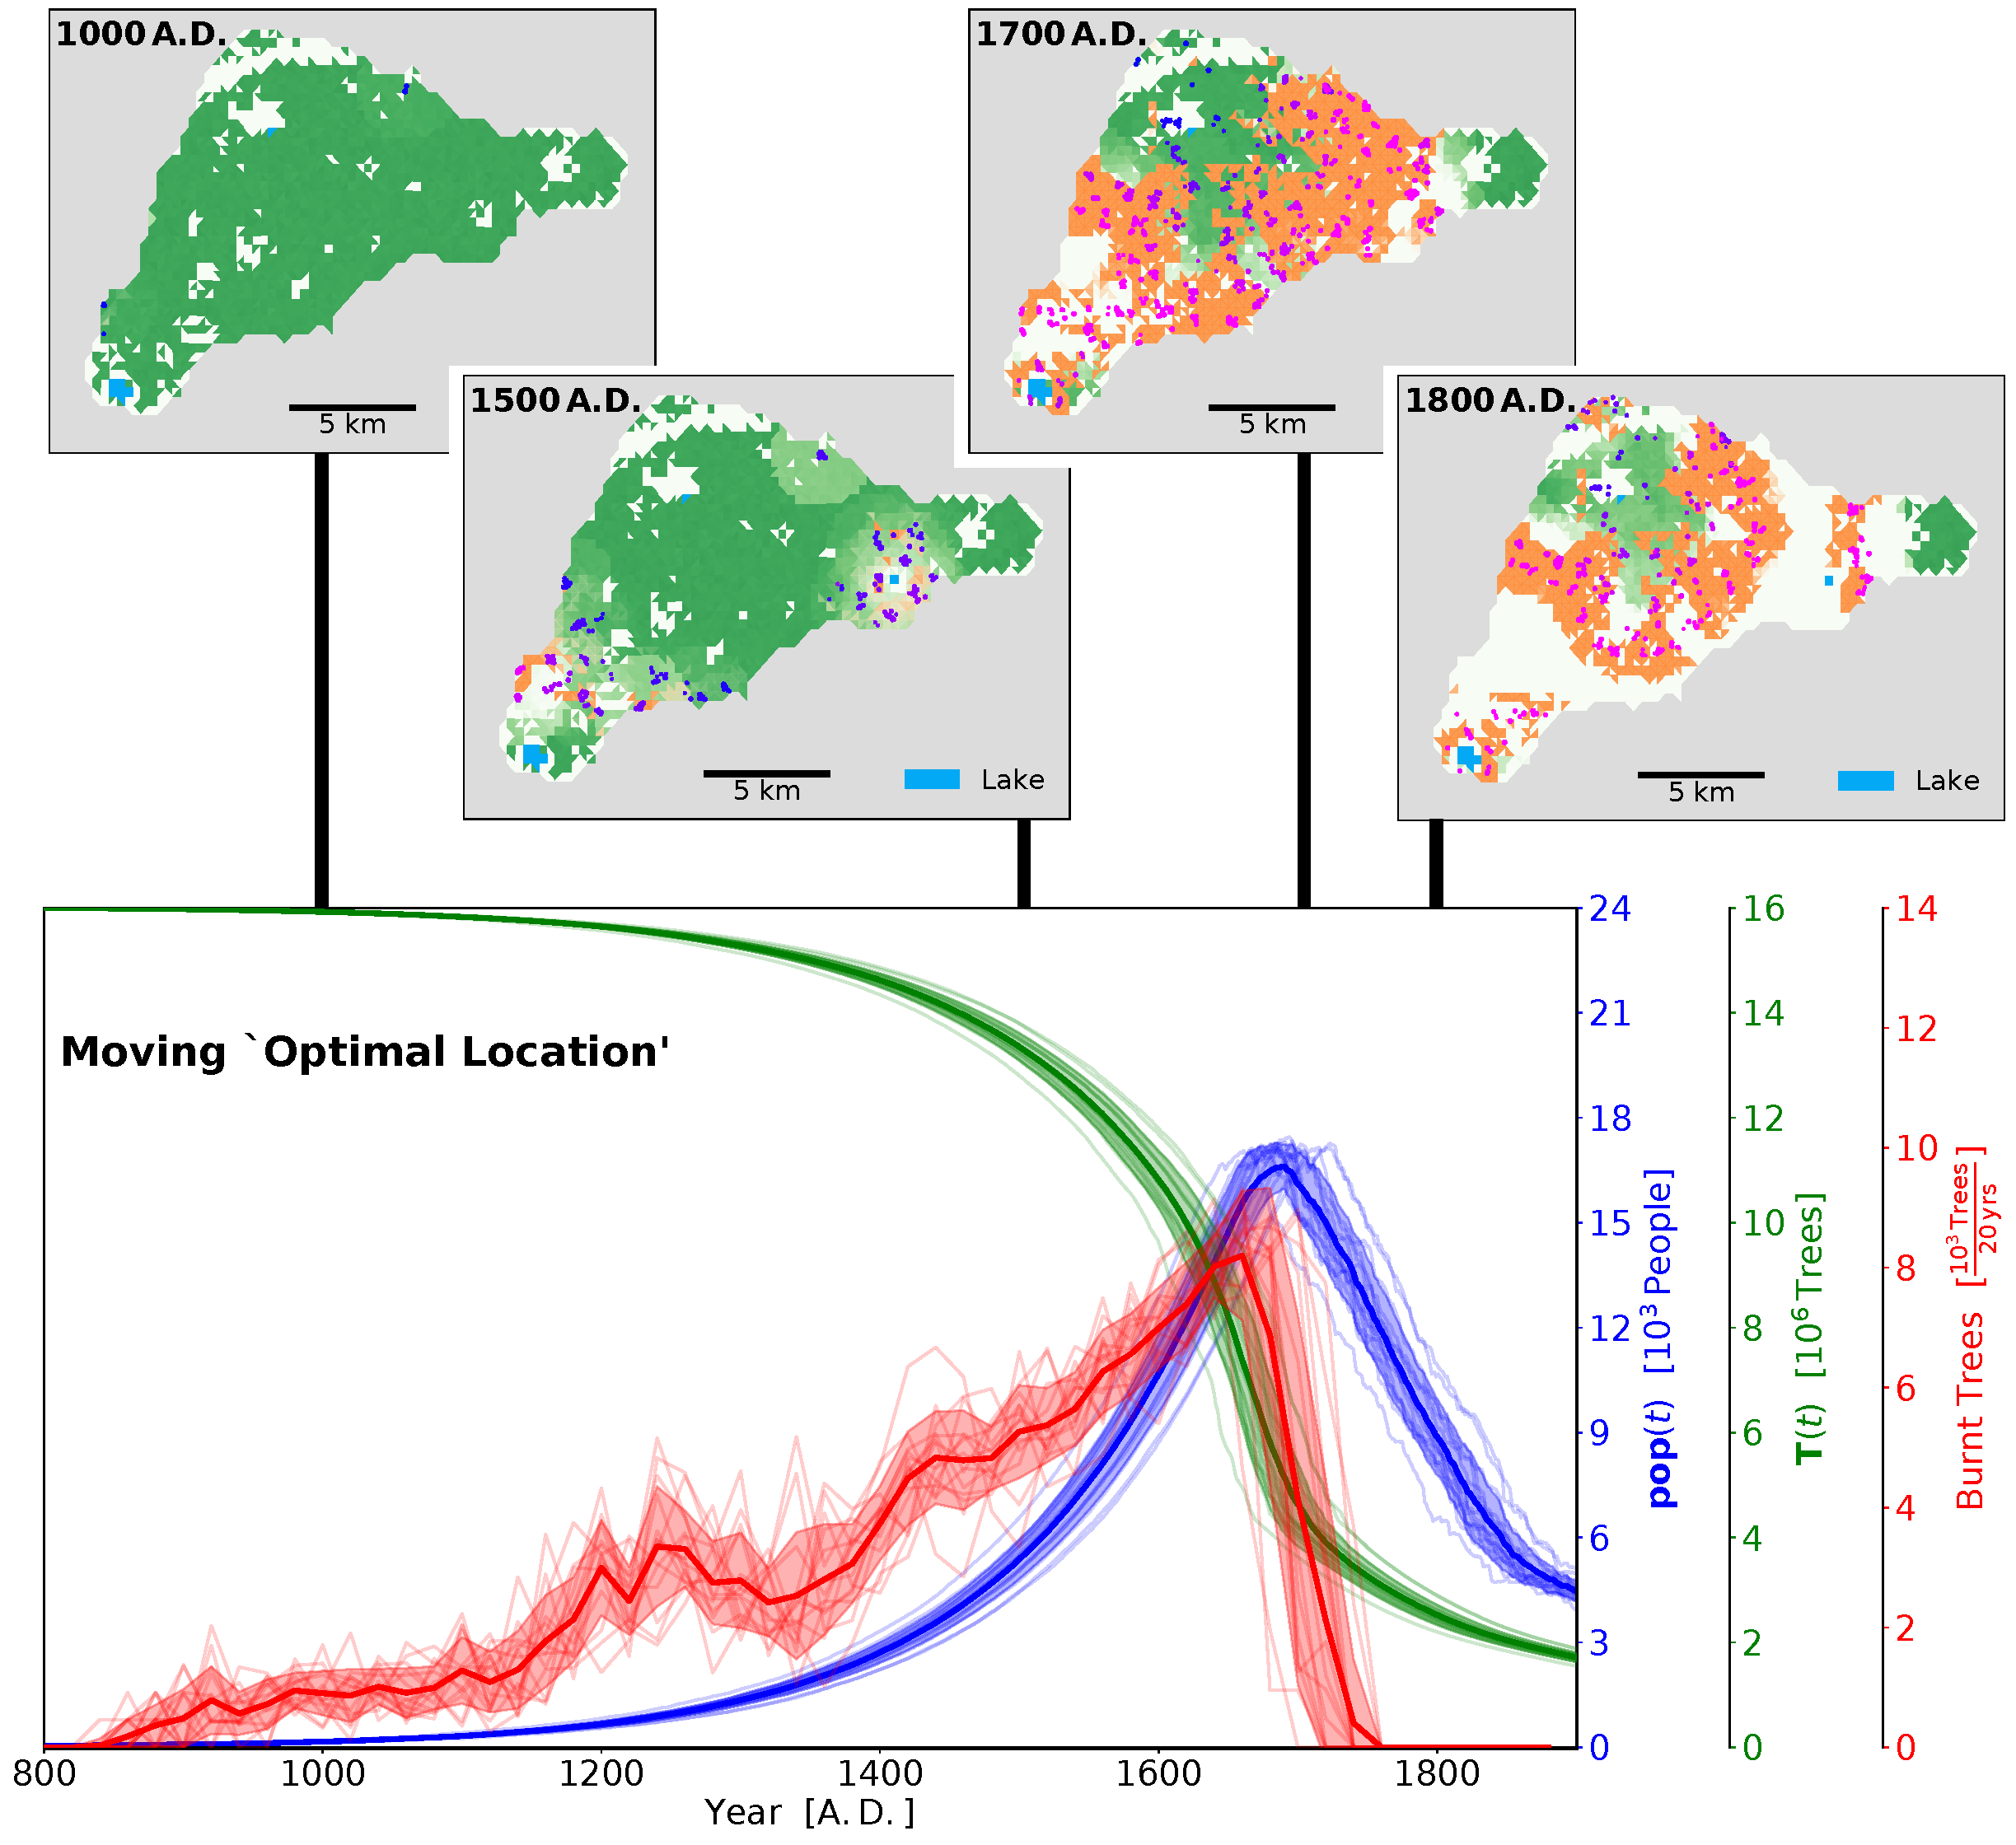
\includegraphics[width=1\textwidth]{images/Results/Moving/alphaDeterministic_EnsembleStatistics+Panels}
	\caption{Moving strategy `Optimal Location'.}
	\label{fig:optimal}
\end{figure}
\begin{figure}
	\centering
	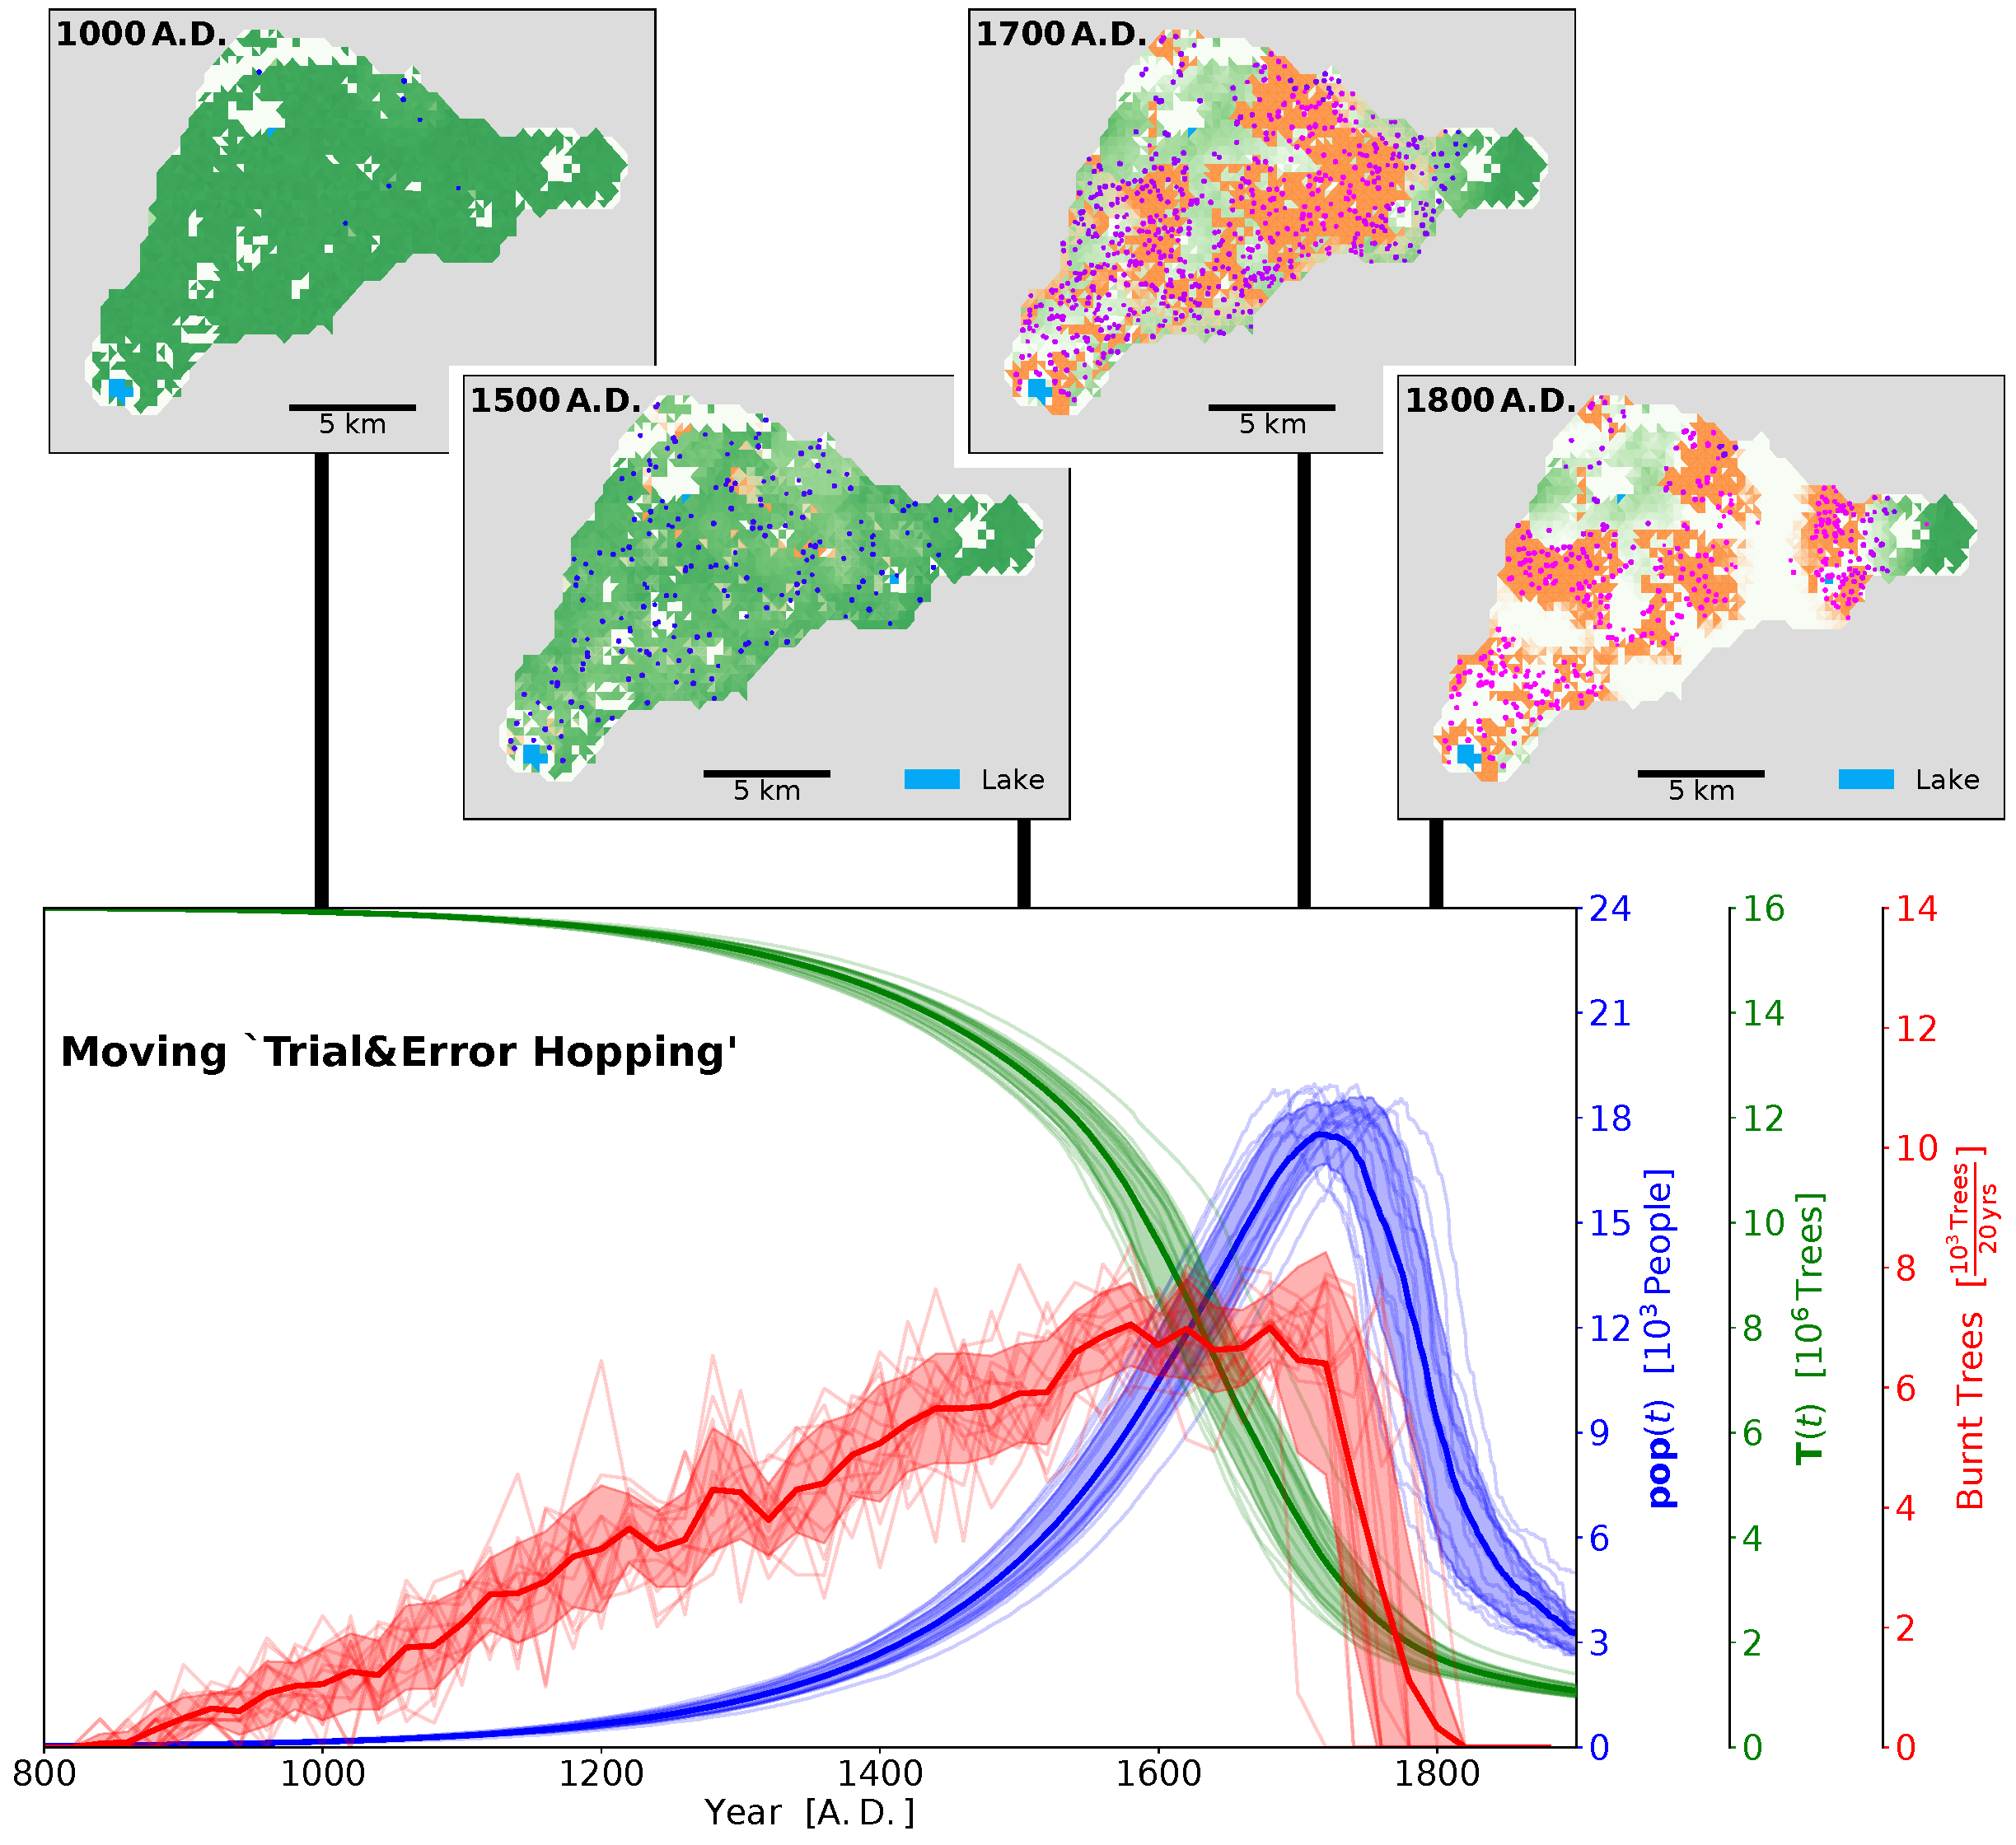
\includegraphics[width=1\textwidth]{images/Results/Moving/alphaHopping_EnsembleStatistics+Panels}
	\caption{Moving strategy `Trial\&Error Hopping'.}
	\label{fig:hop}
\end{figure}
The four different moving strategies presented here (Standard, Only Resources, Optimal Location and Trial\&Error Hopping) do not only change the spatial pattern but also influence the overall dynamics of the model and, therefore, can not be simply computationally reduced in the calculation of aggregate variables,
This is especially apparent for the number of burnt trees.
In particular, if agents do not move according to considerations (`Trial\&Error Hopping' strategy), the overall population dynamics are affected, e.g.\ the decrease after the population size peak becomes steeper.
%\section{Fires}
%Plot the distribution of fires on the map over time. 
%I imagine a map in which the color determines the timing of fires in each cell. 
%I'm not sure yet how to do this exactly since fires in any cell occur at multiple times. Maybe I'll take the first occurence. We'll see.



%The choice of penalty contributions and their functional dependency is described in the remaining Section.
\paragraph{Comment on the Moving Module.}
There is, of course, substantial freedom in modelling the evaluations of potential new locations and the decision making process in the moving module.
The framework is therefore kept flexible and other assumptions or new categories can easily be added or adjusted.
There has not been any comparable approach for Easter Island society yet.
In the ABM simulating the Anasazi people from \citet{Axtell2002} and \citet{Janssen2009}, agents that relocate their farms (and settlements) consider all eligible cells that fulfil certain nutrient production and water availability criteria and then choose the cell closest to the previous location.
In general, I use a similar rationale but implement a more elaborate evaluation process that in particular introduces non-linear, continuous rather than binary evaluation criteria, more/different penalty categories and stochasticity in the decision making process.  
As shown, this procedure (in the standard setting) yields interesting moving patterns which are consistent with plausible beliefs on Easter Island history.



